\documentclass[12pt,a4paper]{article}

% ---------------- Packages ----------------
\usepackage[utf8]{inputenc}      % Hỗ trợ mã UTF-8 cho tiếng Việt
\usepackage[vietnamese]{babel}   % Quy tắc văn bản tiếng Việt
\usepackage{enumitem}            % custom bullet
\usepackage{graphicx}            % Chèn hình ảnh
\usepackage{amsmath, amssymb}    % Công thức toán học nâng cao
\usepackage{fancyhdr}            % Tùy chỉnh header/footer
\usepackage{xcolor}              % Tạo màu sắc cho văn bản/code
\usepackage{geometry}            % Tùy chỉnh lề trang
\usepackage{hyperref}            % Tạo hyperlink và link mục lục
\usepackage{float}               % Hỗ trợ tùy chọn float [H]
\geometry{a4paper, margin=2.5cm}


% ---------------- Header & Footer ----------------
\fancyhf{}
\setlength{\headheight}{15pt}

\lhead{Nhóm 4 - 23KDL1}
\rhead{\thepage}

\pagestyle{fancy}

% ================== THÊM CHO PHẦN CLASS / METHOD ==================
% Hộp đẹp cho Class
\usepackage[most]{tcolorbox}

% Font Helvetica (không bắt buộc, chỉ để cảm giác hiện đại hơn)
\usepackage{helvet}

% Màu sắc theo "theme" kiểu Scikit-learn
\definecolor{sklearn-orange}{RGB}{248, 153, 29}
\definecolor{sklearn-blue}{RGB}{52, 113, 163}
\definecolor{code-bg}{RGB}{245, 245, 245}

% Hộp Class
\newtcolorbox{classbox}[1]{
    breakable, 
    colback=white,
    colframe=sklearn-blue,
    coltitle=white,
    fonttitle=\bfseries\large,
    title=Class: #1,
    boxrule=1pt,
    arc=4pt,
    left=5pt, right=5pt, top=5pt, bottom=5pt,
    before skip=10pt, after skip=10pt
}

% Danh sách Method
\newenvironment{methodlist}{
    \begin{description}[style=nextline, font=\ttfamily\color{sklearn-blue}]
}{
    \end{description}
}
% ================== HẾT PHẦN THÊM ==================

% ---------------- Document Start ----------------
\begin{document}

% ----------- Tiêu đề -----------
\begin{center}
    {\Large \textbf{Báo cáo đồ án cuối khóa}}\\[0.3cm]
    {\large Python cho Khoa học dữ liệu / Dự đoán khối lượng chất béo}\\[1cm]
\end{center}

% ----------- Mục lục tự động -----------
\tableofcontents
\newpage

% ----------- Nội dung báo cáo -----------
\section{Giới thiệu bài toán và dữ liệu}
\label{sec:intro_dataset}

Trong project này, bài toán được lựa chọn là \textbf{hồi quy (regression)}, với mục tiêu dự đoán \textbf{lượng khối lượng chất béo của các món ăn nhanh} tại những chuỗi cửa hàng lớn, dựa trên các đặc trưng dinh dưỡng của từng sản phẩm.

\noindent Bộ dữ liệu sử dụng là \textit{Fast\_Food\_Dataset}, được công bố trên Kaggle\footnote{\url{https://www.kaggle.com/datasets/tan5577/nutritonal-fast-food-dataset}}.

\subsection{Mô tả dữ liệu và EDA}

Dưới đây là mô tả chi tiết các trường dữ liệu có trong bộ dữ liệu, được thể hiện trong Bảng~\ref{tab:data_description}.

\begin{table}[H]
\centering
\begin{tabular}{|l|p{10cm}|}
\hline
\textbf{Cột} & \textbf{Mô tả} \\ \hline
Company & Tên công ty hoặc thương hiệu cung cấp sản phẩm. \\ \hline
Item & Tên món ăn hoặc sản phẩm cụ thể. \\ \hline
Calories & Tổng lượng calo trong một khẩu phần. \\ \hline
Calories from Fat & Lượng calo có nguồn gốc từ chất béo. \\ \hline
Total Fat (g) & Tổng lượng chất béo (gram) trong một khẩu phần. \\ \hline
Saturated Fat (g) & Lượng chất béo bão hòa (gram). \\ \hline
Trans Fat (g) & Lượng chất béo chuyển hóa (gram). \\ \hline
Cholesterol (mg) & Hàm lượng cholesterol (mg). \\ \hline
Sodium (mg) & Hàm lượng natri/muối (mg). \\ \hline
Carbs (g) & Tổng lượng carbohydrate (gram). \\ \hline
Fiber (g) & Hàm lượng chất xơ (gram). \\ \hline
Sugars (g) & Lượng đường (gram). \\ \hline
Protein (g) & Hàm lượng protein (gram). \\ \hline
Weight Watchers Pnts & Điểm số theo hệ thống đánh giá dinh dưỡng Weight Watchers. \\ \hline
\end{tabular}
\caption{Bảng mô tả dữ liệu Fast\_Food\_Dataset}
\label{tab:data_description}
\end{table}

\begin{figure}[H]
    \centering
    
    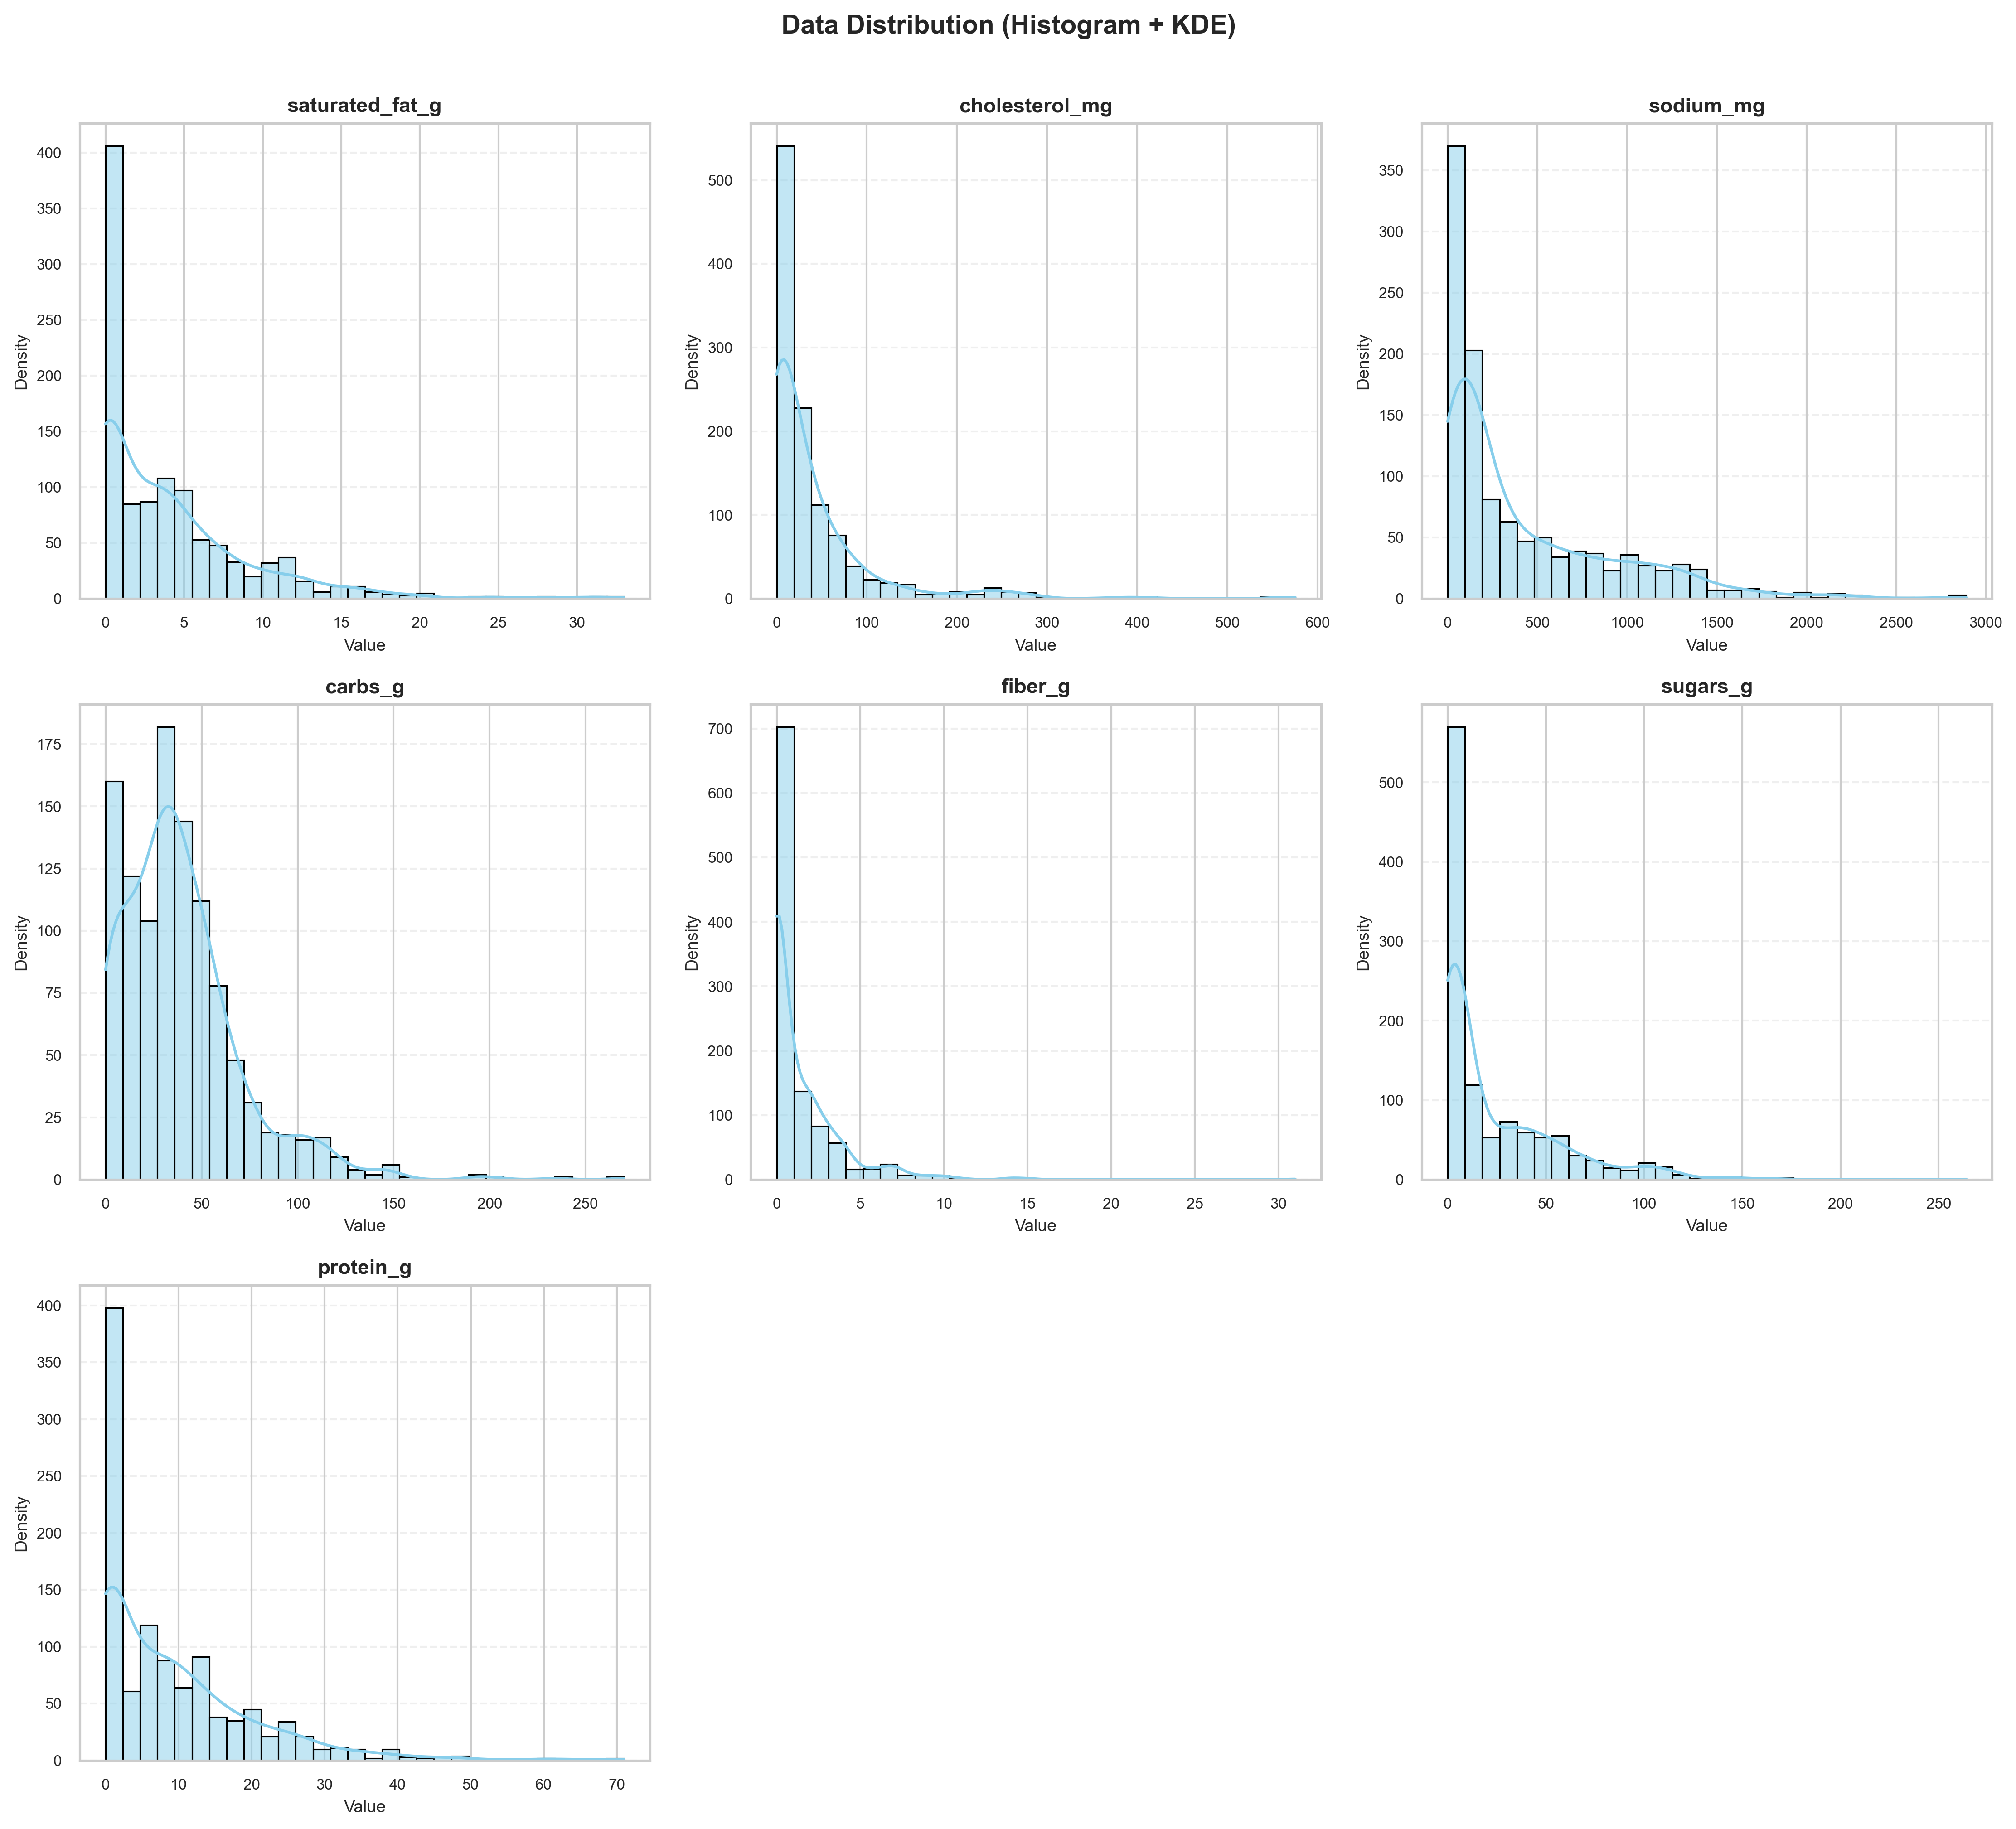
\includegraphics[width=0.75\textwidth]{../../outputs/plots/eda/before/distribution_all.png}
    \caption{Phân phối dữ liệu các đặc trưng}
    \label{fig:distribution}
\end{figure}


\begin{figure}[H]
    \centering
    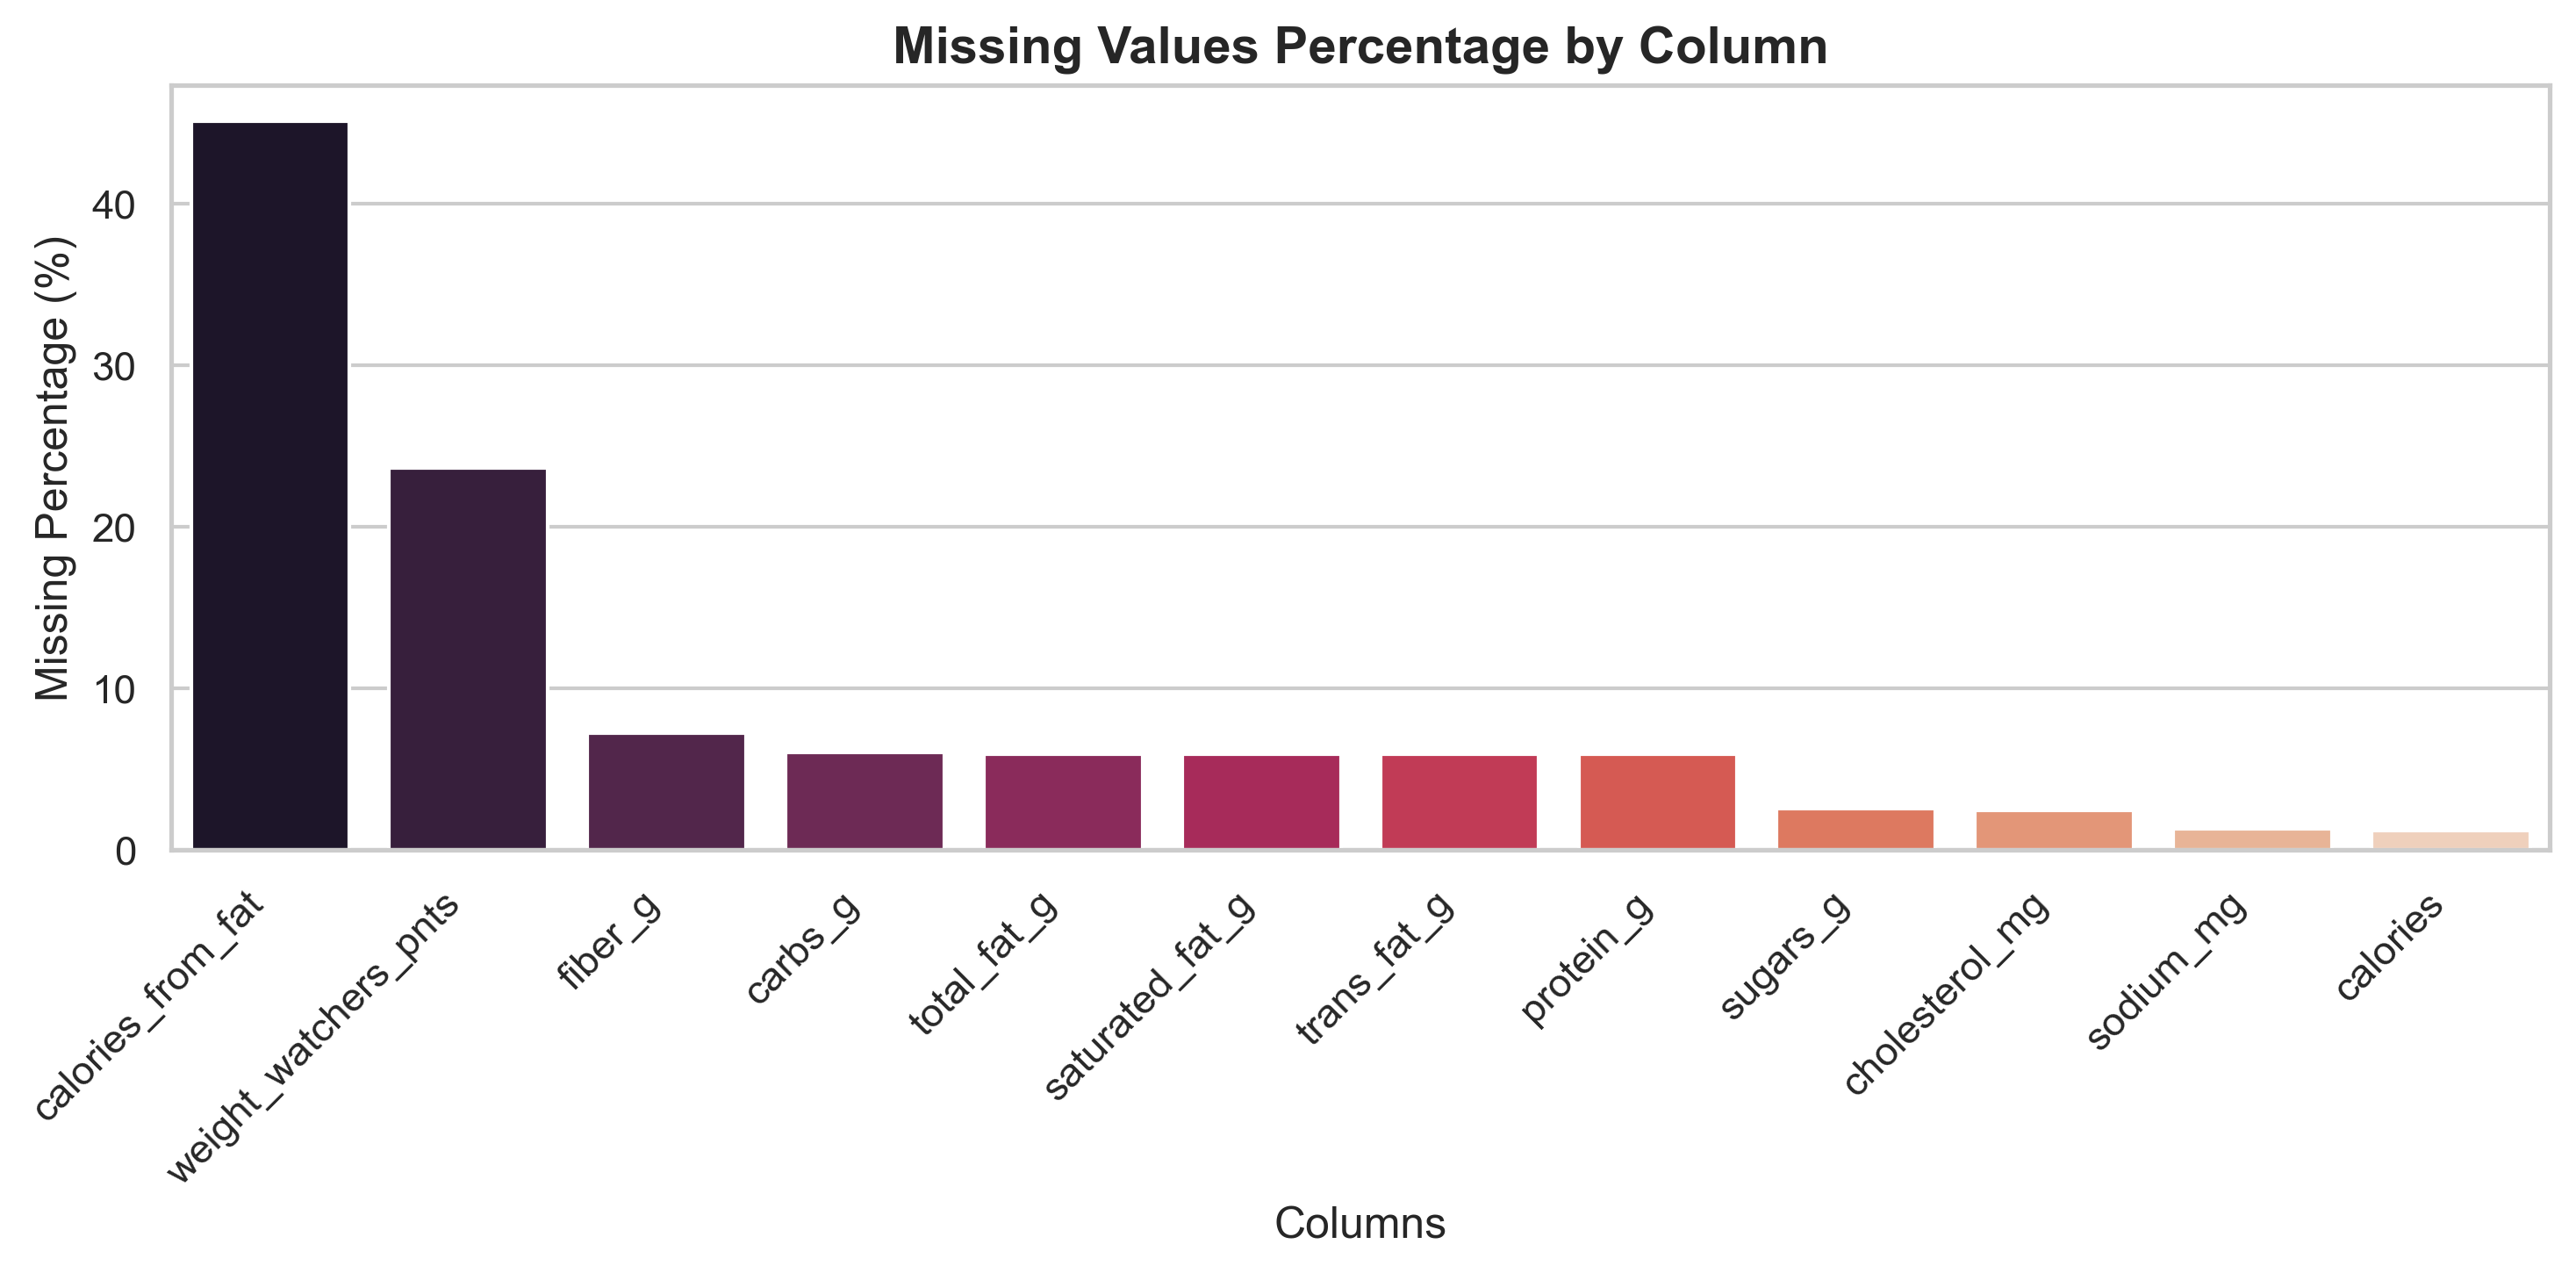
\includegraphics[width=0.75\textwidth]{../../outputs/plots/eda/before/missing_values.png}
    \caption{Biểu đồ giá trị khuyết trong dữ liệu}
    \label{fig:missing}
\end{figure}

\begin{figure}[H]
    \centering
    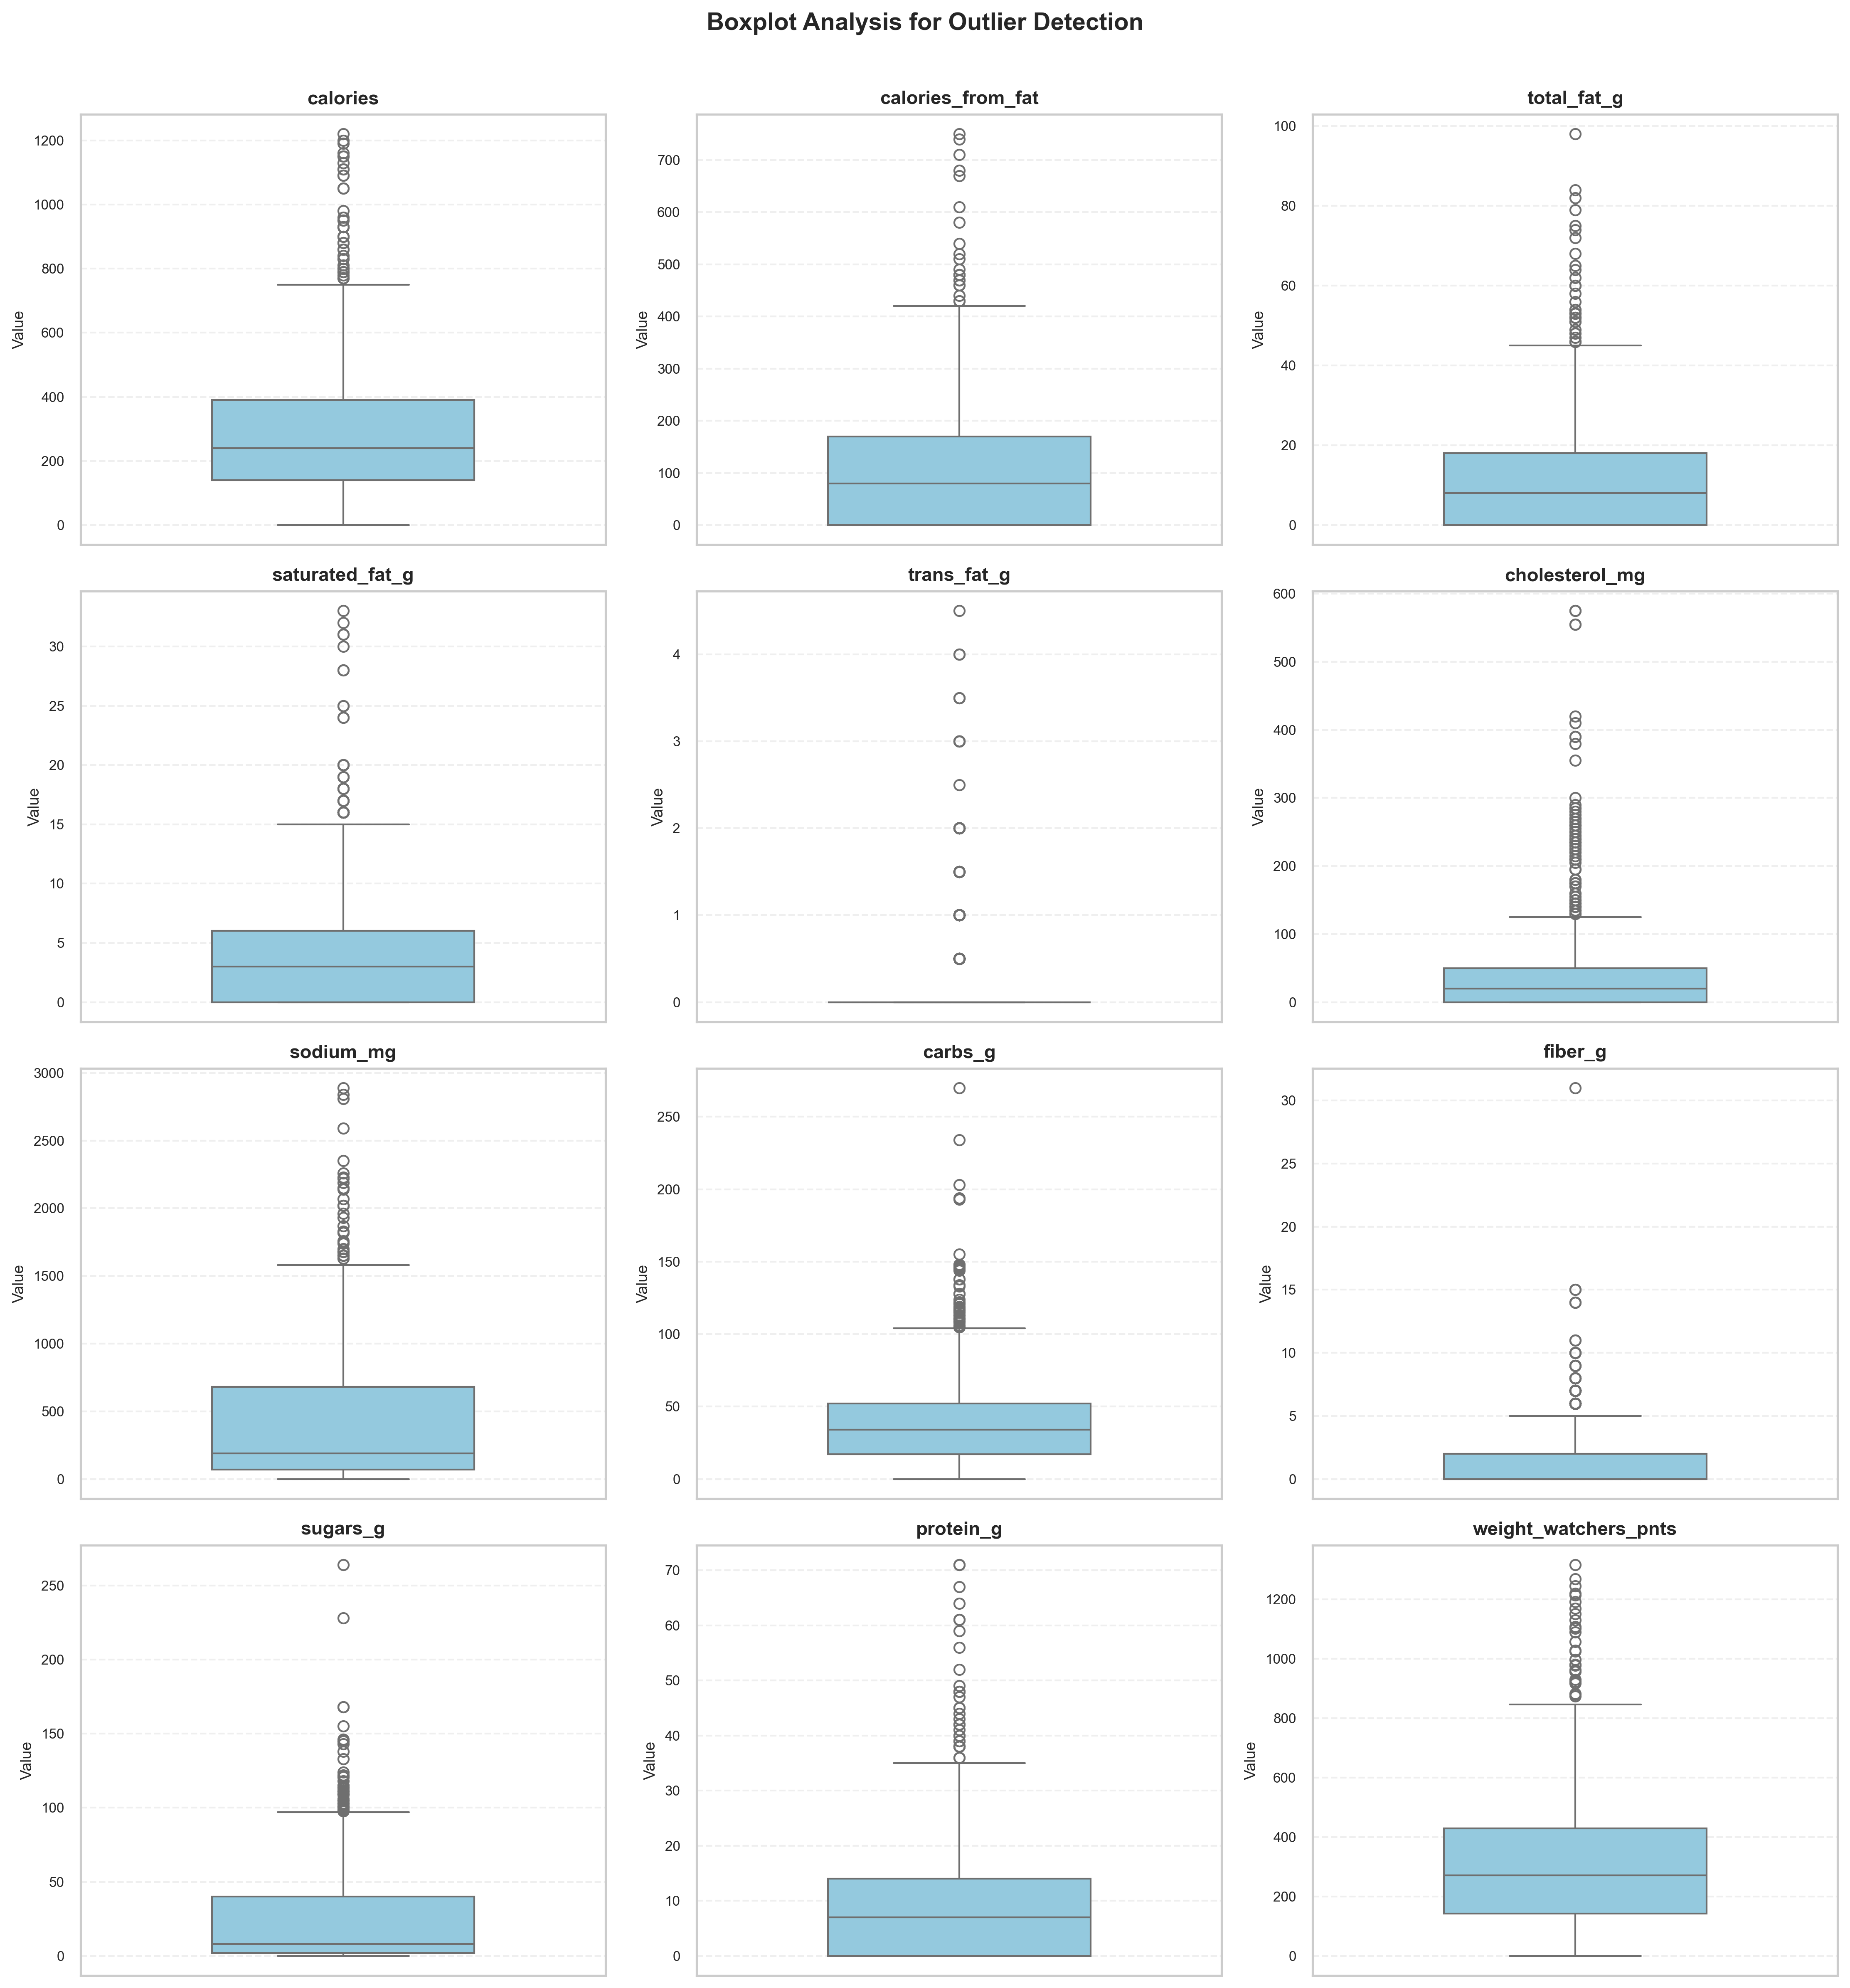
\includegraphics[width=0.7\textwidth]{../../outputs/plots/eda/before/boxplot_all.png}
    \caption{Biểu đồ hộp (boxplot) các đặc trưng}
    \label{fig:boxplot}
\end{figure}

\begin{figure}[H]
    \centering
    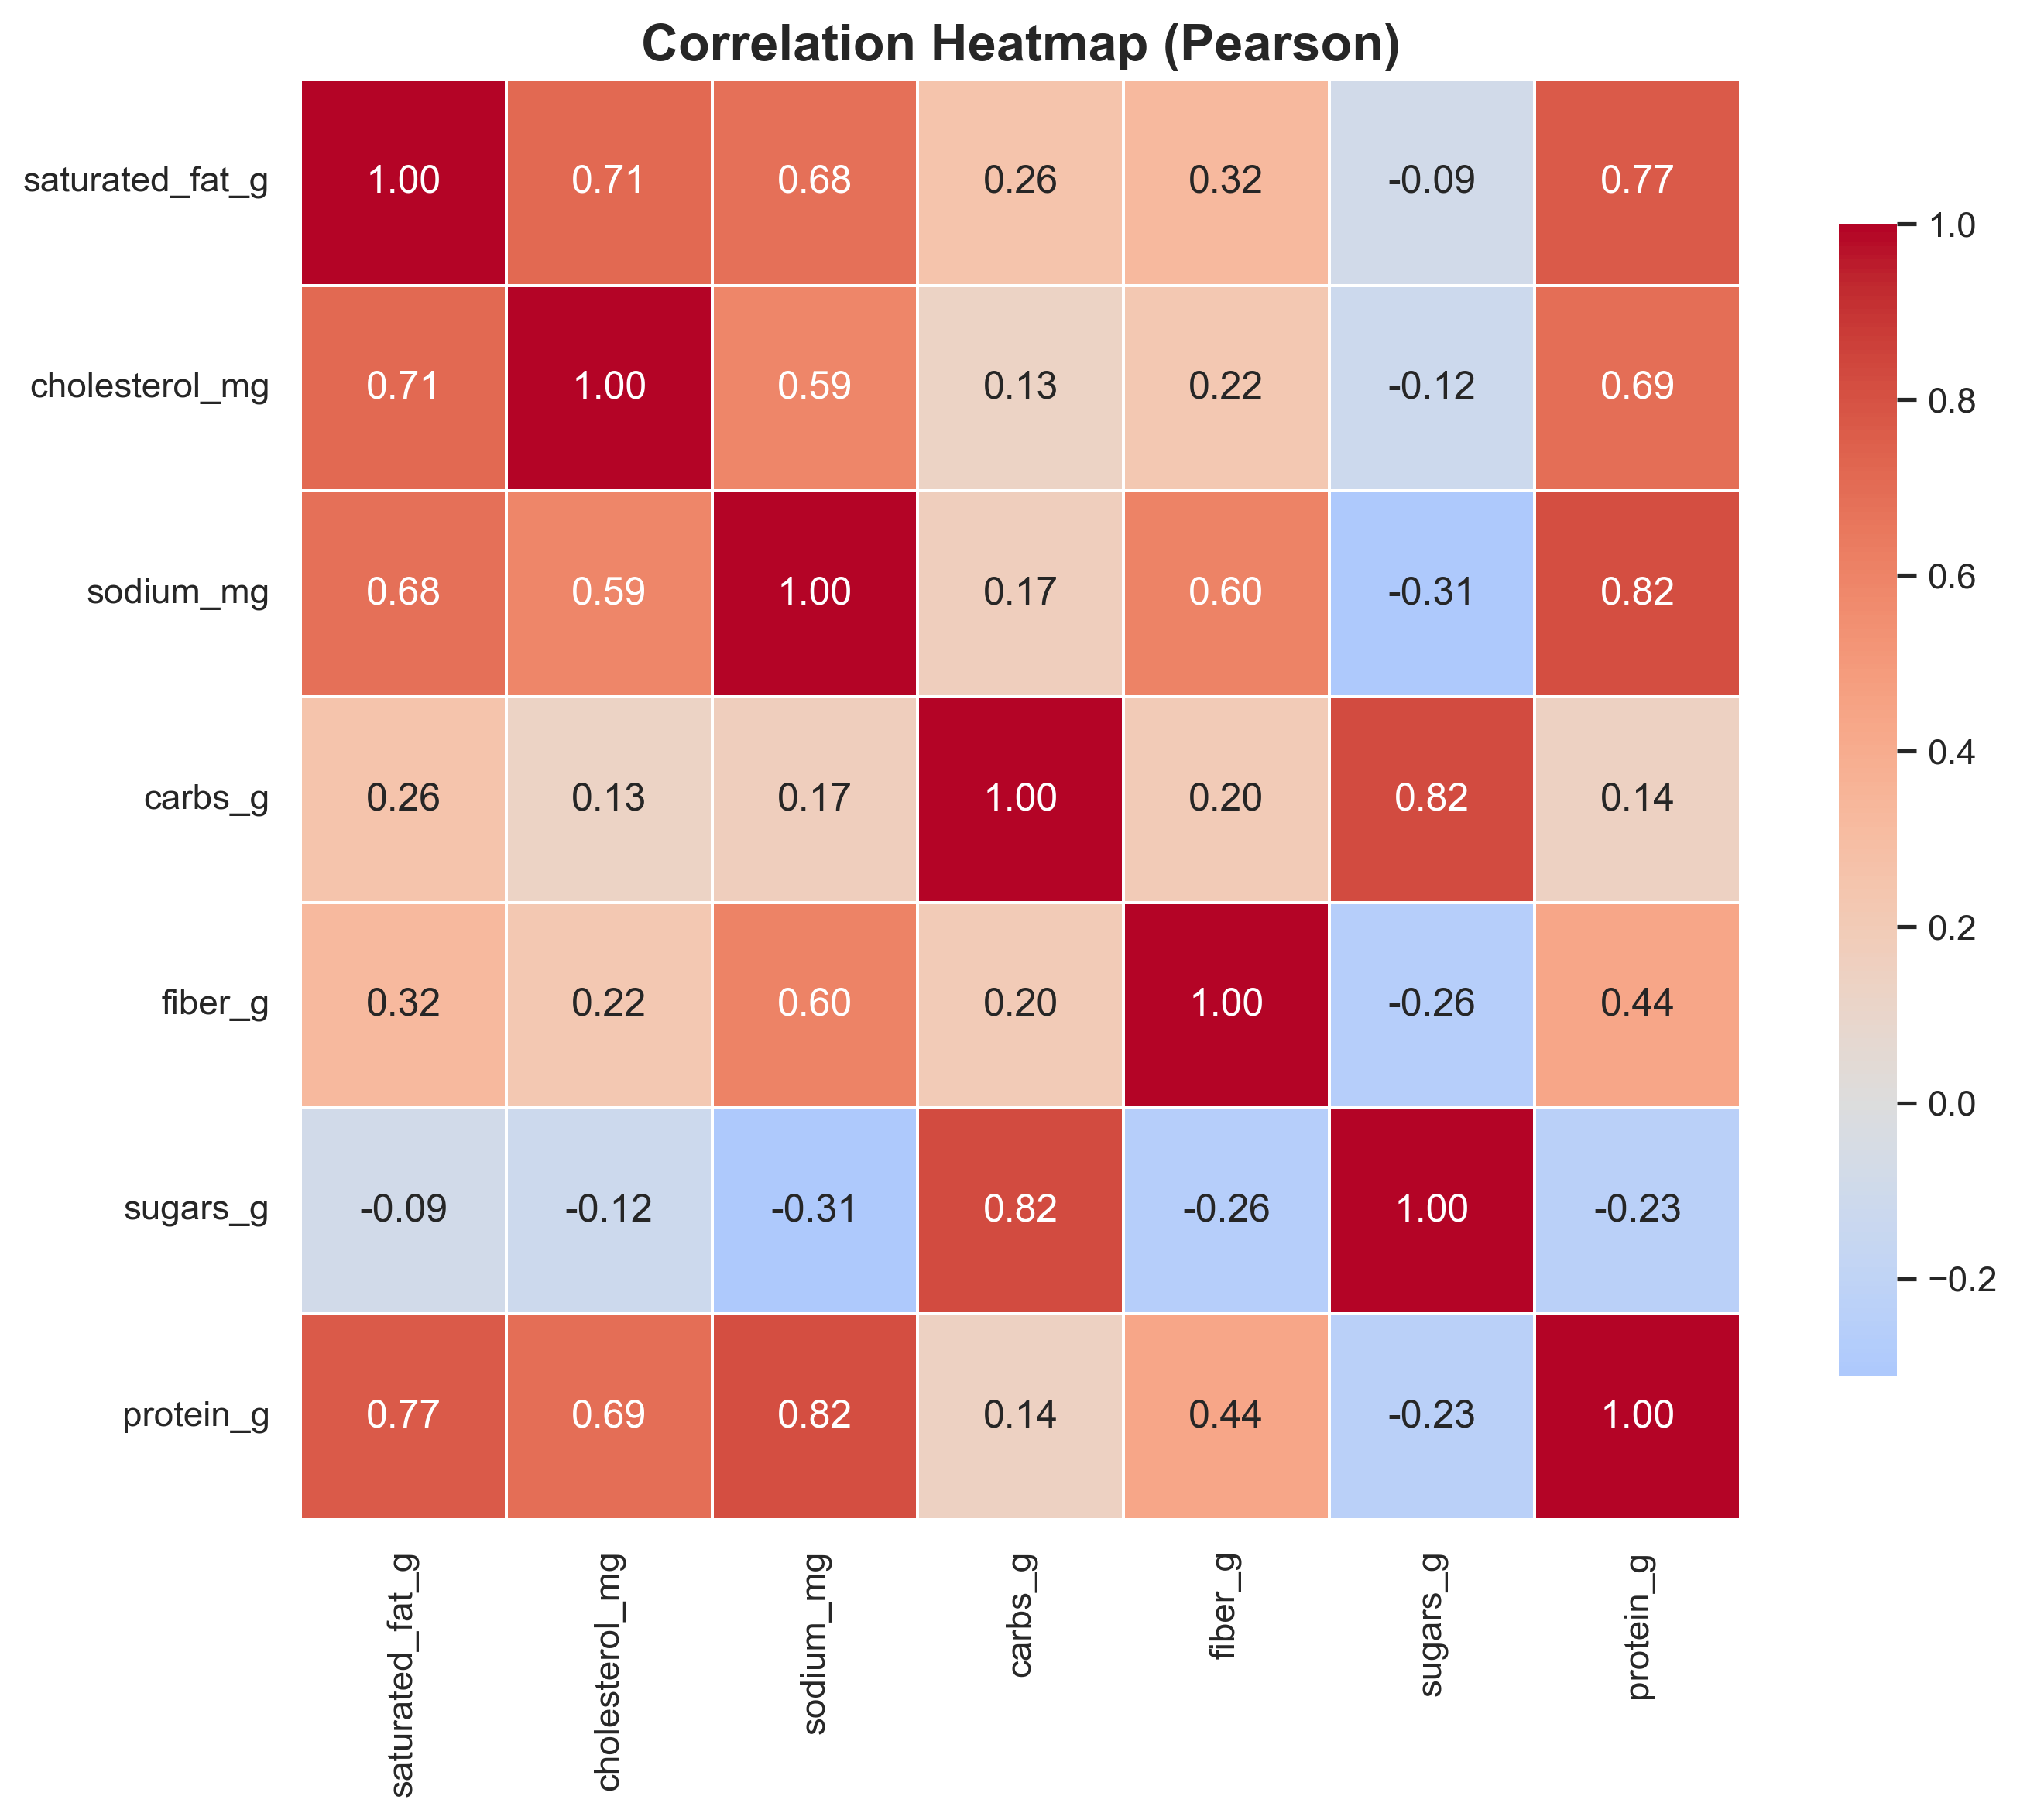
\includegraphics[width=0.7\textwidth]{../../outputs/plots/eda/before/correlation_heatmap_pearson.png}
    \caption{Heatmap tương quan các đặc trưng (Pearson)}
    \label{fig:heatmap_pearson}
\end{figure}

\begin{figure}[H]
    \centering
    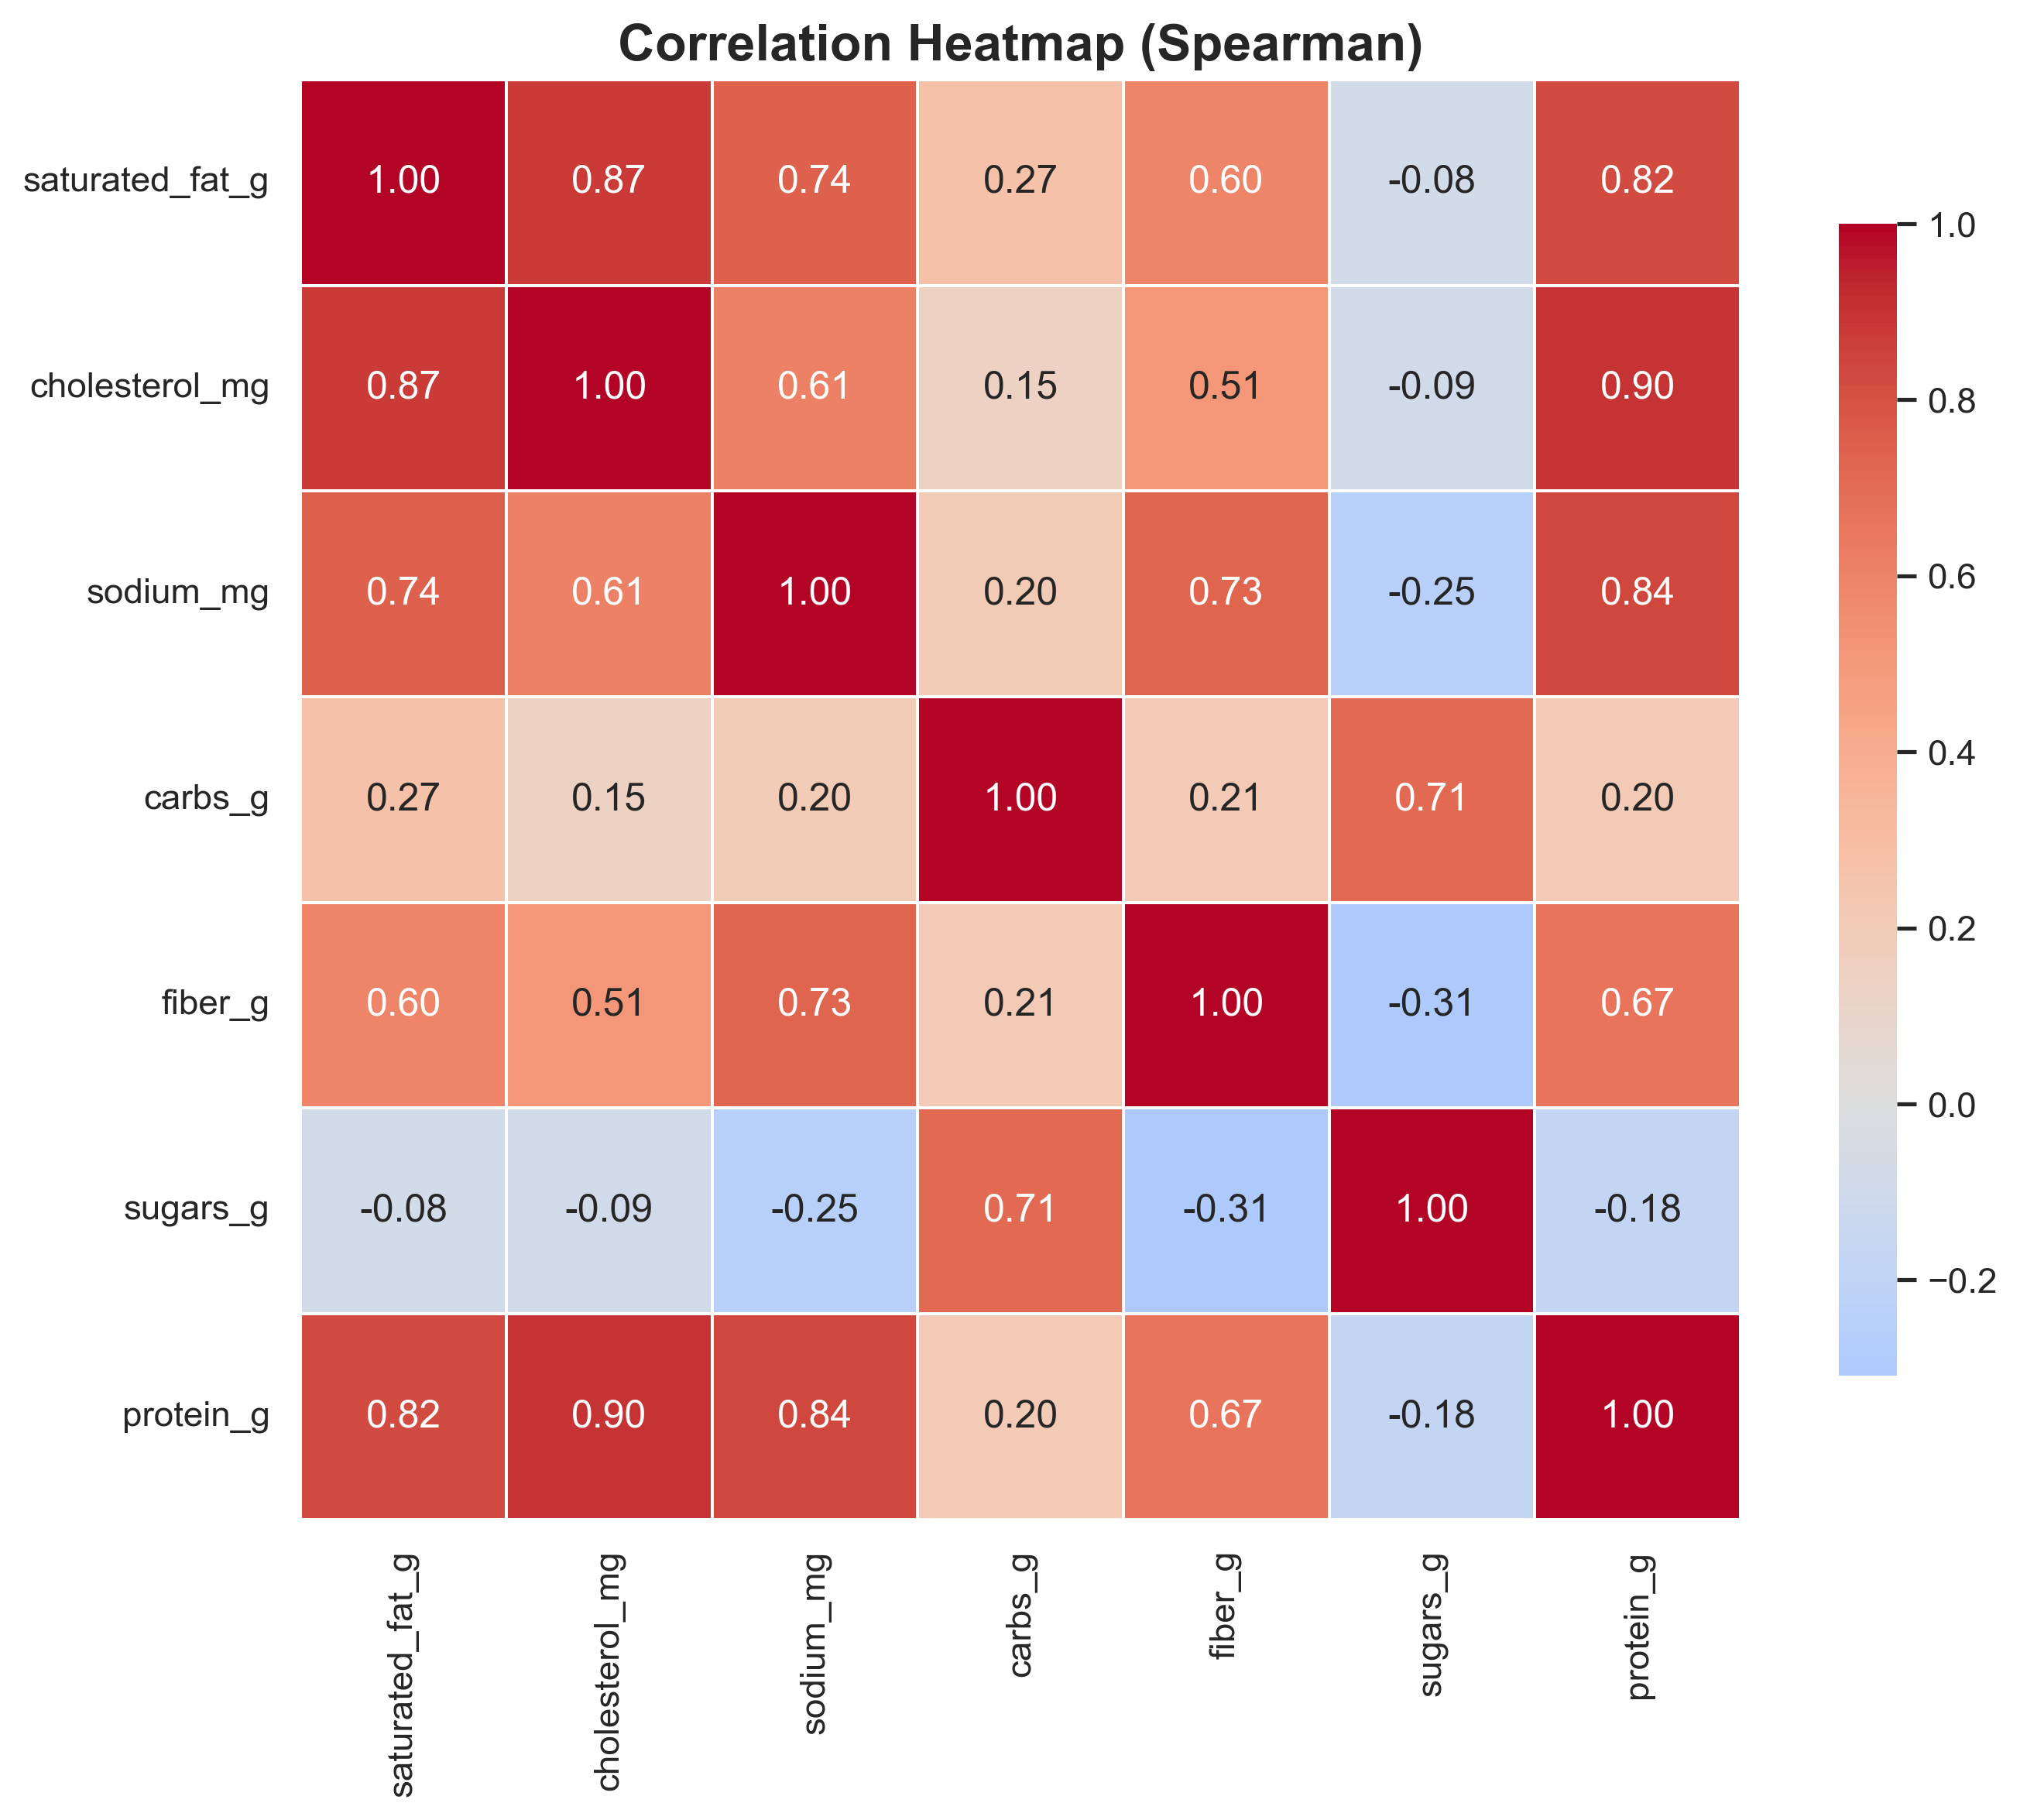
\includegraphics[width=0.7\textwidth]{../../outputs/plots/eda/before/correlation_heatmap_spearman.png}
    \caption{Heatmap tương quan các đặc trưng (Spearman)}
    \label{fig:heatmap_spearman}
\end{figure}

\begin{figure}[H]
    \centering
    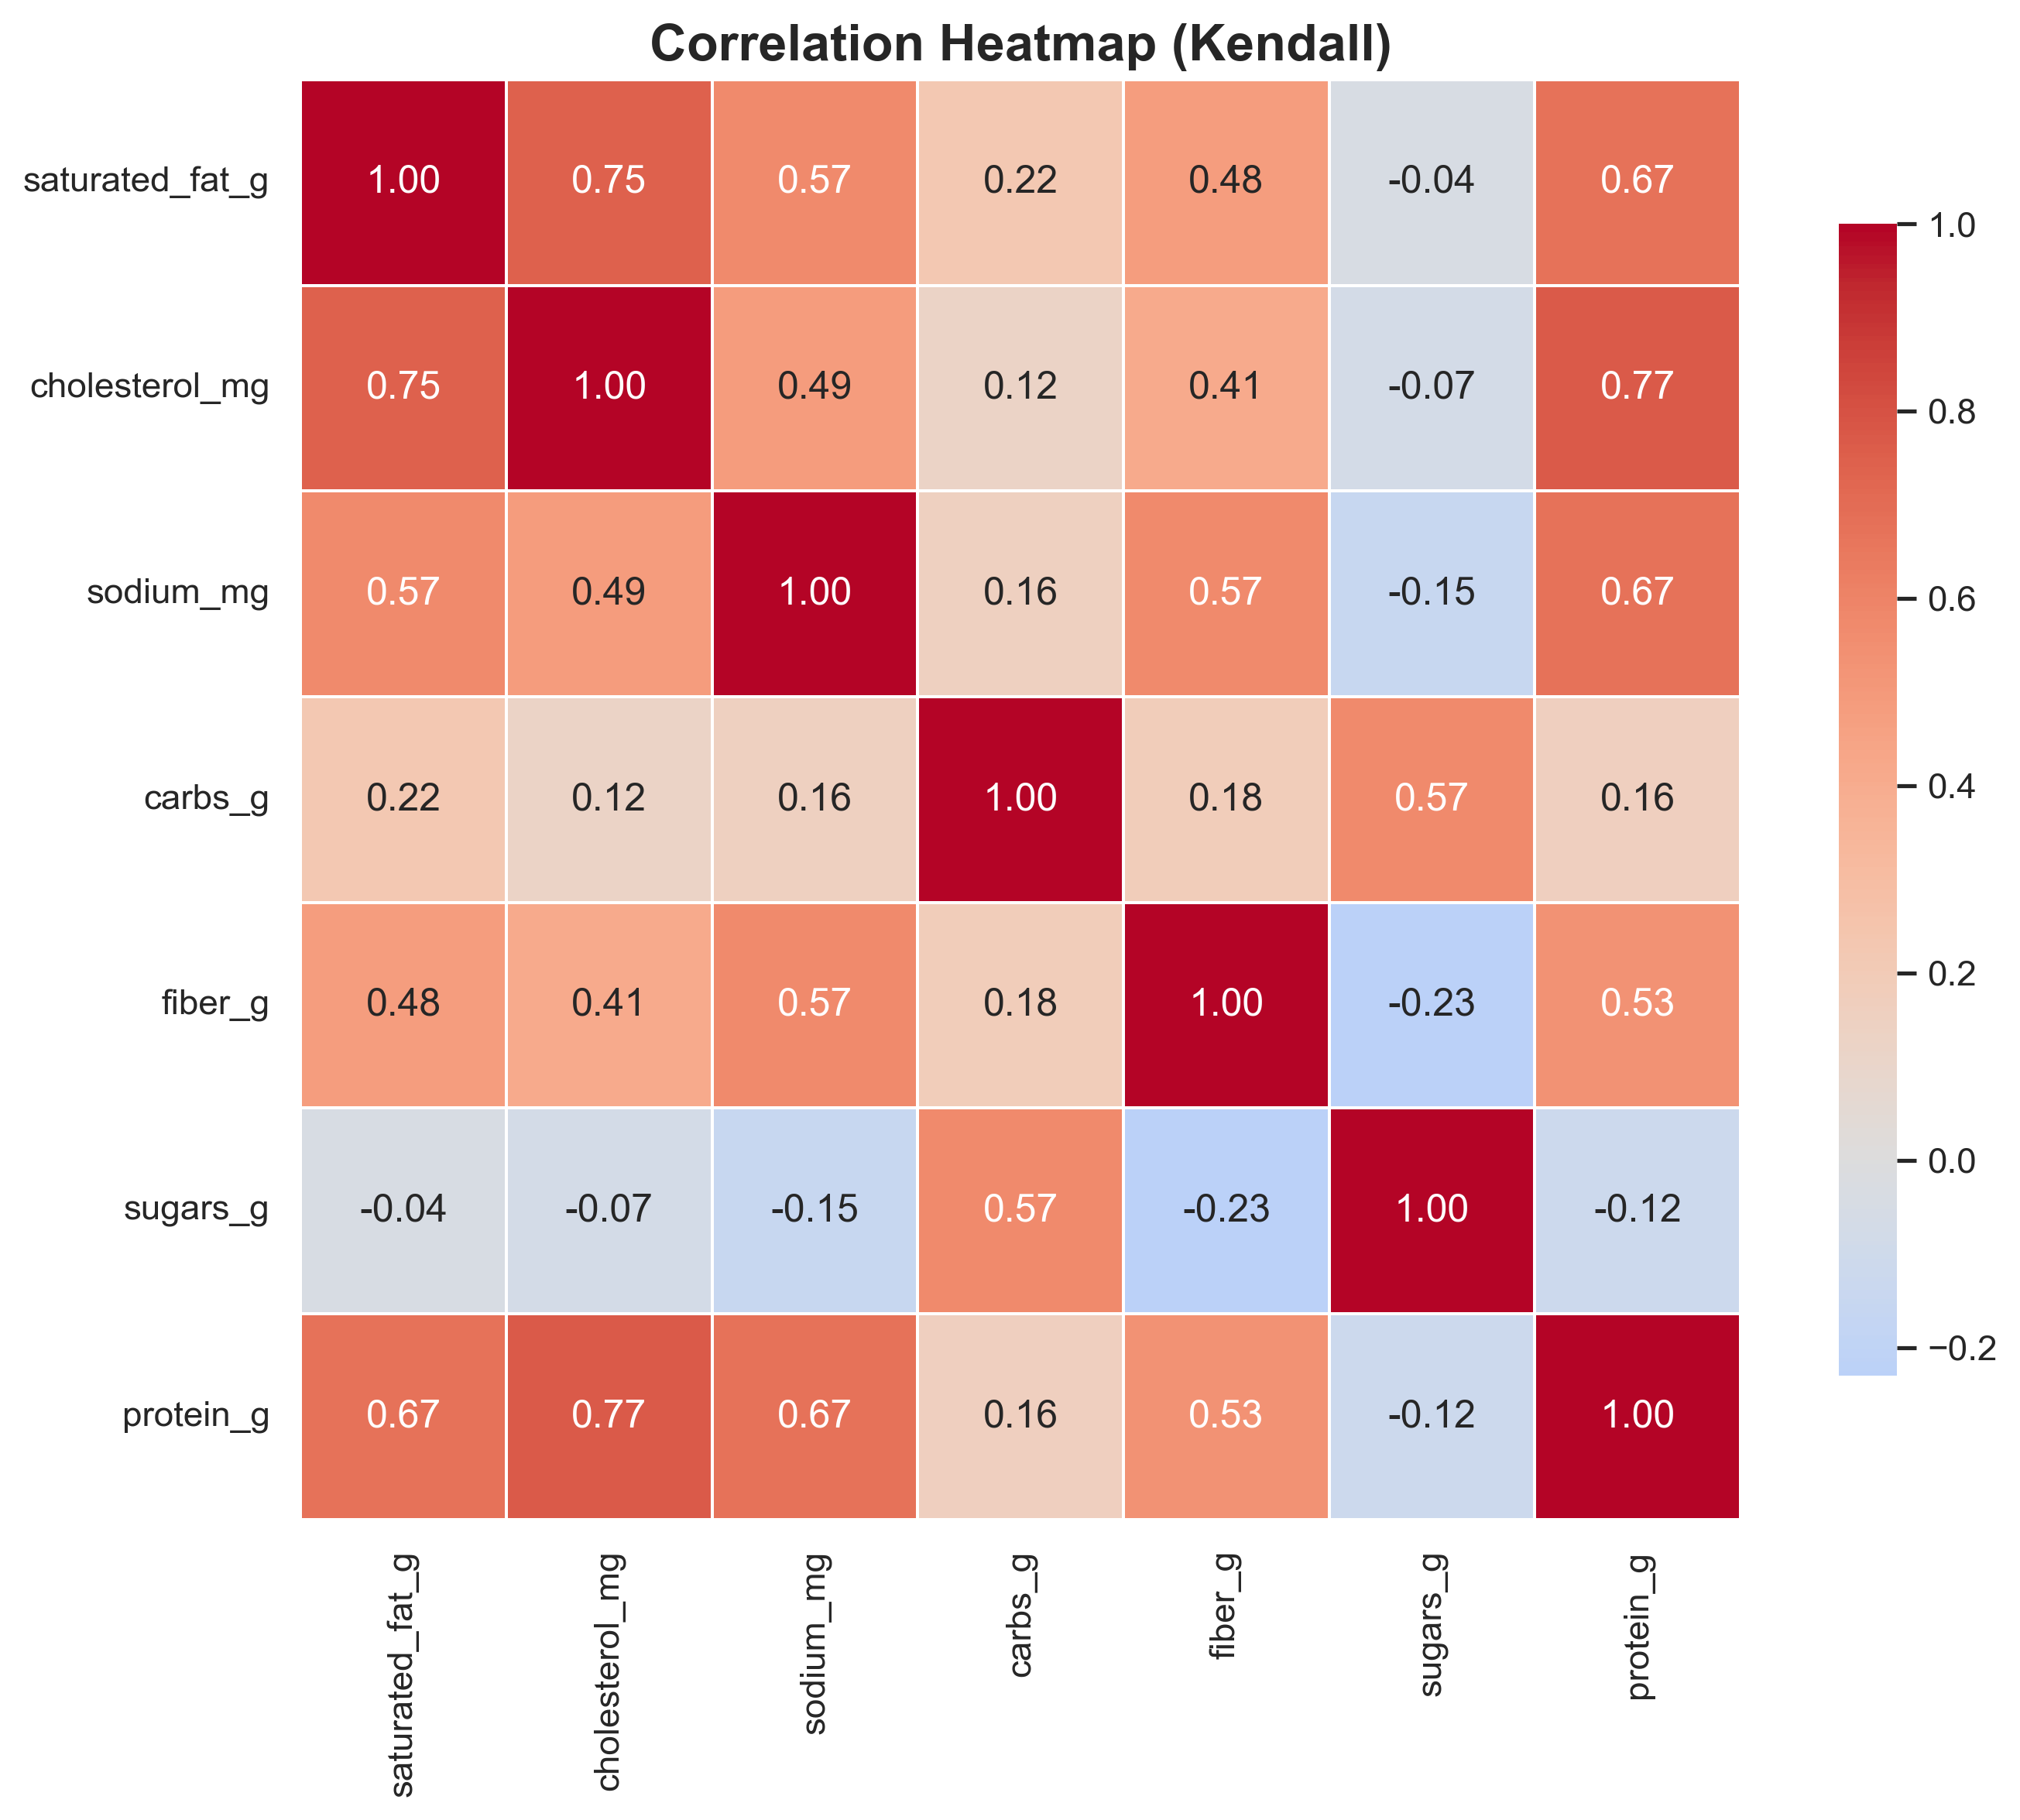
\includegraphics[width=0.7\textwidth]{../../outputs/plots/eda/before/correlation_heatmap_kendall.png}
    \caption{Heatmap tương quan các đặc trưng (Kendall)}
    \label{fig:heatmap_kendall}
\end{figure}

\subsection{Phân tích dữ liệu}
\indent \indent Bộ dữ liệu này có phân phối lệch phải với toàn bộ đặc trưng, chứa khá nhiều giá trị ngoại lai (outliers), ta sẽ phải xem xét để quyết định áp dụng các phương pháp xử lý phù hợp.

Hình~\ref{fig:missing} minh họa số lượng giá trị khuyết trong từng đặc trưng, điều đáng chú ý là cột mục tiêu \textbf{saturated\_fat\_g} cũng có một lượng giá trị khuyết, ta sẽ phải bỏ các hàng bị thiếu này đi, ngoài ra khi xem xét kĩ hơn, các hàng này đều chứa giá trị thiếu ở các đặc trưng của nó.

Dựa trên heatmap tương quan ở Hình~\ref{fig:heatmap_pearson}, Hình~\ref{fig:heatmap_spearman} và Hình~\ref{fig:heatmap_kendall}, ta rút được một số nhận xét quan trọng sau:

\begin{itemize}
    \item \textbf{cholesterol\_mg}, \textbf{sodium\_mg} và \textbf{protein\_g} là các đặc trưng có tương quan cao nhất với mục tiêu.
    \item Đặc trưng \textbf{protein\_g} có tương quan khá cao với các đặc trưng khác, điều này có thể dẫn tới đa colinearity, ảnh hưởng tới hiệu năng mô hình.
\end{itemize}

Dựa trên ngữ nghĩa thực tế, ta sẽ \textbf{chuyển toàn bộ giá trị âm thành giá trị dương} (nếu có tại đây chính là lỗi nhập liệu—typo).

\subsection{Ý nghĩa thực tiễn của bài toán}

Việc ước lượng hàm lượng chất béo xấu (bao gồm \textit{saturated fat} và \textit{trans fat}) từ các chỉ số dinh dưỡng dễ thu thập như \textit{cholesterol}, \textit{sodium} (dựa vào nhãn thành phần), \textit{carbohydrate}, \textit{fiber}, \textit{sugars} và \textit{protein} (có thể cân dễ dàng ở nhà) mang lại nhiều ý nghĩa thực tiễn quan trọng trong đời sống hằng ngày, đặc biệt trong bối cảnh người dùng phổ thông không có điều kiện đo lường chính xác các thành phần chất béo bằng thiết bị chuyên dụng.

\subsubsection{Đối với người nội trợ}

\begin{itemize}
    \item Ước lượng nhanh mức độ chất béo xấu trong bữa ăn hằng ngày.
    \item Điều chỉnh lượng gia vị, dầu mỡ và các thực phẩm có nguồn gốc động vật.
    \item Chủ động bảo vệ sức khỏe tim mạch cho các thành viên trong gia đình.
\end{itemize}

\subsubsection{Đối với người ăn kiêng và người tập luyện}

\begin{itemize}
    \item Duy trì tỷ lệ mỡ cơ thể ở mức hợp lý.
    \item Hạn chế nguy cơ rối loạn mỡ máu trong quá trình ăn kiêng kéo dài.
    \item Tối ưu hoá hiệu quả tập luyện thông qua chế độ dinh dưỡng lành mạnh.
\end{itemize}
Mô hình dự đoán giúp nhóm đối tượng này kiểm soát chất béo một cách chủ động ngay cả khi không có sẵn thông tin chi tiết trên nhãn thực phẩm.

\subsubsection{Đối với người bình thường có nhu cầu theo dõi sức khỏe}

Đối với người trưởng thành bình thường, việc duy trì lượng \textit{saturated fat} trong giới hạn khuyến nghị (dưới 10\% tổng năng lượng mỗi ngày, lý tưởng dưới 7\%) giúp giảm đáng kể nguy cơ mắc các bệnh tim mạch, cao huyết áp và tiểu đường type 2. Hệ thống ước lượng từ mô hình học máy có thể:
\begin{itemize}
    \item Cảnh báo sớm khi lượng chất béo xấu vượt ngưỡng an toàn.
    \item Hỗ trợ người dùng điều chỉnh khẩu phần ăn hợp lý theo từng ngày.
    \item Hình thành thói quen ăn uống khoa học và bền vững.
\end{itemize}

\subsubsection{Ứng dụng trong tương lai}

\begin{itemize}
    \item Thực hiện triển khai trên các ứng dụng điện thoại.
    \item Hỗ trợ tích hợp tính toán Cholesterol và Sodium nhanh hơn thay vì phải tìm kiếm nhập liệu thủ công.
\end{itemize}


\section{Giới thiệu các Class và phương thức trong project}
\label{sec:class_methods}

Phần này mô tả cấu trúc mã nguồn của project và giải thích \textbf{chức năng của từng Class cùng các phương thức (methods) chính}. 
Hệ thống được tổ chức trong thư mục \texttt{src/} và chia thành ba package chính:
\textbf{src.data}, \textbf{src.models} và \textbf{src.visualization}. 
Cách trình bày được thiết kế theo phong cách tài liệu kỹ thuật, giúp người đọc dễ dàng tra cứu khi muốn xem lại luồng xử lý của chương trình.

\subsection{Package: src.data}

Package này chịu trách nhiệm xử lý dữ liệu đầu vào, bao gồm: đọc/ghi file, làm sạch dữ liệu thô, xử lý giá trị khuyết, ngoại lai và chuẩn hoá dữ liệu để đưa vào mô hình học máy.

\subsubsection{src/data/io.py}

\begin{classbox}{DataIO}
Class chuyên trách việc Đọc/Ghi file và chuẩn hóa tên cột. 
Đảm bảo dữ liệu được nạp vào và lưu ra đúng định dạng, nhất quán với toàn bộ pipeline.

\vspace{0.2cm}
\textbf{Methods:}
\begin{methodlist}
    \item[load\_data(filepath)] 
    Nạp dữ liệu từ các file (CSV, XLSX, JSON) vào \texttt{pandas DataFrame}. 
    Hỗ trợ xử lý lỗi khi file không tồn tại hoặc sai định dạng, giúp chương trình không bị crash đột ngột.
    
    \item[save\_data(data, filepath)] 
    Lưu \texttt{DataFrame} hiện tại vào file CSV tại đường dẫn chỉ định. 
    Được dùng sau khi dữ liệu đã qua xử lý để lưu lại phiên bản \emph{sạch}.
    
    \item[clean\_column\_names(data)] 
    Chuẩn hóa tên cột: loại bỏ ký tự đặc biệt, khoảng trắng thừa và chuyển về dạng \texttt{snake\_case} để thuận tiện cho việc code và tương thích với các hàm xử lý tiếp theo.
\end{methodlist}
\end{classbox}

\subsubsection{src/data/transformer.py}

\begin{classbox}{DataTransformer}
Class chứa các thuật toán cốt lõi để xử lý dữ liệu như: xử lý giá trị thiếu, xử lý ngoại lai, chuẩn hóa, mã hóa, và chuyển đổi kiểu dữ liệu.
\texttt{DataTransformer} hoạt động ở dạng các hàm thuần (pure functions) trên \texttt{DataFrame}.

\vspace{0.2cm}
\textbf{Methods:}
\begin{methodlist}
    \item[auto\_detect\_columns(data)] 
    Tự động phát hiện và phân loại các cột theo nhóm: \textit{numeric}, \textit{categorical}, \textit{datetime}. 
    Thông tin này được dùng để quyết định chiến lược tiền xử lý phù hợp cho từng loại cột.
    
    \item[convert\_columns\_to\_numeric(data, columns)] 
    Ép kiểu các cột được chỉ định thành kiểu số (int/float), xử lý các ký tự không hợp lệ (ví dụ: dấu phẩy, ký hiệu đơn vị...).
    
    \item[auto\_convert\_numeric\_columns(data, threshold)] 
    Tự động rà soát các cột kiểu \texttt{object} và cố gắng chuyển sang kiểu số. 
    Nếu tỉ lệ giá trị chuyển đổi thành công vượt \texttt{threshold}, cột đó sẽ được coi là cột số.
    
    \item[convert\_to\_datetime(data, columns, date\_format)] 
    Chuyển đổi các cột được chỉ định sang kiểu \texttt{datetime} theo định dạng ngày tháng cung cấp, hỗ trợ chuẩn hóa dữ liệu thời gian.
    
    \item[clean\_negative\_values(data)] 
    Thay thế tất cả giá trị âm trong các cột số bằng giá trị tuyệt đối của chúng. 
    Điều này bám sát quyết định xử lý ở Mục~\ref{sec:intro_dataset}, vì các chỉ số dinh dưỡng không nên mang giá trị âm.
    
    \item[handle\_missing\_values(data, strategies, ...)] 
    Xử lý giá trị thiếu theo chiến lược cấu hình (điền bằng \texttt{mean}, \texttt{median}, \texttt{mode} hoặc \texttt{drop}). 
    Cho phép cấu hình khác nhau cho từng cột hoặc từng nhóm cột.
    
    \item[handle\_outliers(data, method, ...)] 
    Phát hiện và xử lý các giá trị ngoại lai trong cột số sử dụng các phương pháp như \texttt{IQR}, \texttt{Z-score} hoặc \texttt{Isolation Forest}, phù hợp với phần mô tả ở Hình~\ref{fig:boxplot}.
    
    \item[encode\_categorical(data, strategy)] 
    Mã hóa các biến phân loại thành dạng số để mô hình có thể sử dụng (hỗ trợ \texttt{Label Encoding} và \texttt{One-Hot Encoding}).
    
    \item[scale\_features(data, strategy, ...)] 
    Chuẩn hóa dữ liệu số về cùng một khoảng (sử dụng \texttt{StandardScaler} hoặc \texttt{RobustScaler}), khớp với các chiến lược scaling đã trình bày trong Bảng~\ref{tab:top5_preprocess}.
    
    \item[remove\_duplicates(data, subset)] 
    Kiểm tra và loại bỏ các hàng trùng lặp hoàn toàn hoặc trùng trên một tập cột con (\texttt{subset}), giúp giảm nhiễu.
    
    \item[drop\_features(data, features)] 
    Loại bỏ hoàn toàn các cột không cần thiết hoặc đã được xác định là gây ra \textit{data leakage}.
\end{methodlist}
\end{classbox}

\subsubsection{src/data/preprocessor.py}

\begin{classbox}{DataPreprocessor}
Class đóng vai trò \textit{orchestrator} (bộ điều phối), kết hợp \texttt{DataIO} và \texttt{DataTransformer} để tạo thành một pipeline xử lý dữ liệu hoàn chỉnh. 
Class này lưu giữ trạng thái của dữ liệu trong quá trình biến đổi.

\vspace{0.2cm}
\textbf{Methods:}
\begin{methodlist}
    \item[\_\_init\_\_(...)] 
    Khởi tạo đối tượng với các tham số cấu hình cho toàn bộ quy trình (chiến lược xử lý missing values, scaling, outlier, encoding...).
    
    \item[load\_data(filepath, ...)] 
    Gọi \texttt{DataIO.load\_data()} để nạp dữ liệu từ file và thực hiện ngay các bước chuẩn hóa sơ bộ như chuẩn hóa tên cột, ép kiểu cơ bản.
    
    \item[save\_data(filepath)] 
    Lưu trạng thái dữ liệu hiện tại (sau khi xử lý) xuống file, giúp tái sử dụng hoặc chia sẻ cho các bước phân tích khác.
    
    \item[auto\_detect\_columns()] 
    Phân loại các cột (numeric, categorical, datetime) và lưu thông tin này vào thuộc tính nội bộ của class.
    
    \item[convert\_to\_datetime(...)] 
    Gọi hàm chuyển đổi ngày tháng và cập nhật lại \texttt{DataFrame} nội bộ.
    
    \item[clean\_negative\_values()] 
    Thực hiện làm sạch giá trị âm trên dữ liệu hiện có, đảm bảo tính hợp lý về mặt ngữ nghĩa dinh dưỡng.
    
    \item[handle\_missing\_values(...)] 
    Thực hiện xử lý giá trị thiếu. 
    Hỗ trợ chế độ \texttt{fit} (học tham số điền trên train set) và \texttt{transform} (áp dụng cùng tham số đó cho test set) để tránh \textit{data leakage}.
    
    \item[handle\_outliers(...)] 
    Loại bỏ hoặc cắt ngưỡng các giá trị ngoại lai theo cấu hình được chỉ định.
    
    \item[encode\_categorical(...)] 
    Mã hóa biến phân loại và lưu trữ các encoder để áp dụng nhất quán cho dữ liệu mới.
    
    \item[scale\_features(...)] 
    Chuẩn hóa dữ liệu số, lưu lại \texttt{scaler} đã \texttt{fit} để dùng cho tập kiểm tra hoặc dữ liệu triển khai thực tế.
    
    \item[remove\_duplicates(...)] 
    Loại bỏ các hàng trùng lặp trên dữ liệu hiện tại.
    
    \item[drop\_features(...)] 
    Xóa các cột không còn cần thiết (ví dụ: \texttt{Calories from Fat}, \texttt{Weight Watchers Pnts}, \texttt{Company}, \texttt{Item} như phân tích ở mục trước).
    
    \item[get\_processed\_data()] 
    Trả về \texttt{DataFrame} kết quả sau khi đã trải qua toàn bộ pipeline tiền xử lý.
\end{methodlist}
\end{classbox}

\subsection{Package: src.models}

Package này quản lý vòng đời của mô hình học máy: từ huấn luyện, tối ưu siêu tham số cho đến đánh giá và lưu mô hình.

\subsubsection{src/models/evaluator.py}

\begin{classbox}{ModelEvaluator}
Class tiện ích (utility) cung cấp các phương thức tĩnh để tính toán các chỉ số đánh giá hiệu quả mô hình.

\vspace{0.2cm}
\textbf{Methods:}
\begin{methodlist}
    \item[evaluate\_model(model, X\_test, y\_test, model\_name)] 
    Dự đoán trên tập test và tính toán các metrics: \texttt{MSE}, \texttt{RMSE}, \texttt{MAE}, \texttt{R\textsuperscript{2}}. 
    Kết quả được trả về dưới dạng \texttt{dict} để dễ lưu trữ và phân tích.
    
    \item[get\_feature\_importance(model, feature\_names, ...)] 
    Trích xuất độ quan trọng của các đặc trưng từ mô hình đã huấn luyện (hỗ trợ cả mô hình tuyến tính và tree-based). 
    Kết quả này liên kết trực tiếp với phần phân tích ở Hình~\ref{fig:lasso_importance}.
\end{methodlist}
\end{classbox}

\subsubsection{src/models/io.py}

\begin{classbox}{ModelIO}
Class chịu trách nhiệm \textit{serialization} (lưu trữ) và \textit{deserialization} (khôi phục) các mô hình và kết quả đánh giá.

\vspace{0.2cm}
\textbf{Methods:}
\begin{methodlist}
    \item[load\_model(filepath, method)] 
    Đọc file mô hình từ ổ cứng và khôi phục thành object Python. 
    Hỗ trợ các phương thức như \texttt{joblib} và \texttt{pickle}.
    
    \item[save\_model(model, model\_name, ...)] 
    Lưu object mô hình xuống file để tái sử dụng sau này, có thể tự động gắn thêm \texttt{timestamp} nếu không chỉ định tên file cụ thể.
    
    \item[save\_results(results, filepath, format)] 
    Xuất kết quả đánh giá (metrics) ra file CSV hoặc JSON, giúp liên kết với file Google Sheets trong Mục~\ref{sec:ket_qua_thuc_nghiem}.
\end{methodlist}
\end{classbox}

\subsubsection{src/models/trainer.py}

\begin{classbox}{ModelTrainer}
Class trung tâm quản lý quy trình huấn luyện, kết nối giữa dữ liệu đã xử lý, các thuật toán mô hình và bước tối ưu siêu tham số.

\vspace{0.2cm}
\textbf{Methods:}
\begin{methodlist}
    \item[\_\_init\_\_(random\_state)] 
    Khởi tạo Trainer với \texttt{random\_state} cố định để đảm bảo tính tái lập (\textit{reproducibility}).
    
    \item[load\_data(data, target\_column)] 
    Nhận dữ liệu đã tiền xử lý và xác định cột mục tiêu \texttt{target\_column} (trong project là \texttt{Calories}).
    
    \item[split\_data(test\_size, stratify)] 
    Chia dữ liệu thành tập Train/Test theo tỉ lệ chỉ định, hỗ trợ \texttt{stratify} nếu cần.
    
    \item[set\_training\_data(train\_processed, test\_processed, ...)] 
    Thiết lập dữ liệu đầu vào (\texttt{X}) và nhãn (\texttt{y}) cho quá trình huấn luyện từ các \texttt{DataFrame} đã xử lý.
    
    \item[initialize\_models()] 
    Khởi tạo danh sách các mô hình sẽ dùng: \texttt{LinearRegression}, \texttt{Ridge}, \texttt{Lasso}, \texttt{ElasticNet}, \texttt{DecisionTree/RandomForest}, \texttt{LightGBM}...
    
    \item[train\_models(models\_to\_train)] 
    Thực hiện vòng lặp \texttt{fit} cho các mô hình được yêu cầu.
    
    \item[optimize\_params(model\_name, ...)] 
    Sử dụng Bayesian Optimization (thông qua Optuna) để tìm bộ siêu tham số tốt nhất cho một mô hình cụ thể.
    
    \item[evaluate\_models()] 
    Đánh giá toàn bộ các mô hình đã huấn luyện trên tập Test và tìm ra mô hình tốt nhất dựa trên \texttt{R\textsuperscript{2}} (kết quả liên quan tới Hình~\ref{fig:compare_models}).
    
    \item[get\_feature\_importance(model\_name, top\_n)] 
    Lấy danh sách các đặc trưng quan trọng nhất ảnh hưởng đến kết quả dự đoán của mô hình đó.
\end{methodlist}
\end{classbox}

\subsubsection{src/models/optimizer.py}

\begin{classbox}{BayesianOptimizer}
Class chuyên biệt thực hiện tối ưu hóa siêu tham số sử dụng thư viện \texttt{Optuna}.

\vspace{0.2cm}
\textbf{Methods:}
\begin{methodlist}
    \item[\_\_init\_\_(X\_train, y\_train, ...)] 
    Khởi tạo Optimizer với dữ liệu huấn luyện và cấu hình Cross-Validation.
    
    \item[optimize(model\_name, n\_trials)] 
    Định nghĩa không gian tìm kiếm (search space) cho từng loại model và chạy quá trình tối ưu hóa để tối đa hóa \texttt{R\textsuperscript{2}} trên tập validation.
\end{methodlist}
\end{classbox}

\subsection{Package: src.visualization}

Package này cung cấp các công cụ trực quan hóa giúp hiểu rõ dữ liệu và kết quả mô hình thông qua các biểu đồ, gắn với các hình đã trình bày ở phần trước.

\subsubsection{src/visualization/eda.py}

\begin{classbox}{EDA}
Class thực hiện \textit{Exploratory Data Analysis} (Phân tích Dữ liệu Khám phá), giúp có cái nhìn tổng quan về dữ liệu trước khi mô hình hóa.

\vspace{0.2cm}
\textbf{Methods:}
\begin{methodlist}
    \item[\_\_init\_\_(data, show\_plots)] 
    Khởi tạo với dữ liệu cần phân tích và cờ \texttt{show\_plots} để quyết định có hiển thị trực tiếp biểu đồ hay chỉ lưu file.
    
    \item[summary\_statistics(save\_path)] 
    Tính toán và hiển thị các thống kê mô tả, kiểm tra giá trị thiếu, trùng lặp và độ lệch (skewness) của dữ liệu.
    
    \item[correlation\_analysis(method, save\_path)] 
    Tính toán ma trận tương quan (Pearson, Spearman...) và vẽ Heatmap, tương ứng với Hình~\ref{fig:heatmap}.
    
    \item[data\_distribution(save\_path)] 
    Vẽ biểu đồ histogram kết hợp đường cong mật độ (KDE) để xem phân phối của từng biến số, như Hình~\ref{fig:distribution}.
    
    \item[boxplot\_analysis(save\_path)] 
    Vẽ boxplot cho các đặc trưng số nhằm trực quan hóa ngoại lệ, như Hình~\ref{fig:boxplot}.
    
    \item[perform\_eda(corr\_method, save\_path)] 
    Phương thức tiện ích chạy toàn bộ quy trình EDA theo trình tự chuẩn: thống kê mô tả, phân phối, tương quan, boxplot...
\end{methodlist}
\end{classbox}

\subsubsection{src/visualization/model\_plots.py}

\begin{classbox}{ModelVisualizer}
Class chuyên biệt để trực quan hóa hiệu năng của các mô hình sau khi huấn luyện.

\vspace{0.2cm}
\textbf{Methods:}
\begin{methodlist}
    \item[\_\_init\_\_(evaluation\_results)] 
    Khởi tạo với kết quả đánh giá thu được từ \texttt{ModelTrainer} (ví dụ: bảng metrics của từng mô hình).
    
    \item[plot\_model\_comparison(save\_path)] 
    Vẽ biểu đồ cột so sánh các chỉ số MSE, RMSE, MAE, R\textsuperscript{2} giữa các mô hình, tương ứng với Hình~\ref{fig:compare_models}.
    
    \item[plot\_feature\_importance(importance\_df, save\_path)] 
    Vẽ biểu đồ thanh ngang thể hiện mức độ đóng góp của từng đặc trưng vào quyết định của mô hình, tương ứng với Hình~\ref{fig:lasso_importance}.
\end{methodlist}
\end{classbox}

\section{Tổng quan thư viện và phương pháp tối ưu siêu tham số}

\subsection{Thư viện học máy sử dụng}
Trong nghiên cứu này, bốn thư viện chính được sử dụng gồm \textbf{Scikit-learn (sklearn)}, \textbf{LightGBM}, \textbf{XGBoost} và \textbf{Optuna}. 

Sklearn là thư viện phổ biến trong Python, cung cấp đầy đủ các thuật toán học máy truyền thống như hồi quy tuyến tính, cây quyết định và các phương pháp đánh giá mô hình. 

LightGBM là thư viện chuyên dụng cho các mô hình cây tăng cường (Gradient Boosting), có tốc độ huấn luyện nhanh và hiệu quả cao với tập dữ liệu lớn. 

XGBoost là thư viện học máy mạnh mẽ dựa trên cây quyết định, nổi tiếng với khả năng xử lý dữ liệu khuyết thiếu và tối ưu hóa hiệu suất tính toán.

Optuna là thư viện tối ưu siêu tham số tự động, hỗ trợ nhiều chiến lược tìm kiếm tiên tiến.

\subsection{Các mô hình được sử dụng}
Các mô hình hồi quy được áp dụng trong nghiên cứu gồm: \textbf{Elastic Net}, \textbf{Decision Tree Regression}, \textbf{Random Forest Regression}, \textbf{LightGBM Regression} và \textbf{XGBoost Regression}. 

Elastic Net là mô hình tuyến tính kết hợp regularization L1 và L2, giúp phân tích mối quan hệ tuyến tính giữa biến đầu vào và đầu ra. 

Các mô hình còn lại thuộc họ cây quyết định (tree-based) có khả năng mô hình hóa quan hệ phi tuyến phức tạp, trong đó Random Forest, LightGBM và XGBoost là các ensemble methods với hiệu suất cao.

\subsection{Chỉ số đánh giá mô hình}
Hiệu quả của các mô hình được đánh giá thông qua ba chỉ số chính: \textbf{R-squared ($R^2$)}, \textbf{Mean Squared Error (MSE)} và \textbf{Mean Absolute Error (MAE)}. 
\begin{itemize}
    \item \textbf{Mean Squared Error (MSE)}: Công thức tính:
    \[MSE = \frac{1}{n} \sum_{i=1}^{n} (y_i - \hat{y}_i)^2\]
    MSE nên được sử dụng khi ta muốn phạt nặng các sai số lớn, tuy nhiên nó bị ảnh hưởng lớn bởi các giá trị ngoại lai.
    \item \textbf{Mean Absolute Error (MAE)}: Công thức tính:
    \[MAE = \frac{1}{n} \sum_{i=1}^{n} |y_i - \hat{y}_i|\]
    MAE nên được sử dụng khi ta muốn đánh giá sai số trung bình.
    \item \textbf{R-squared ($R^2$)}: Công thức tính:
    \[R^2 = 1 - \frac{\sum_{i=1}^{n} (y_i - \hat{y}_i)^2}{\sum_{i=1}^{n} (y_i - \bar{y})^2}\]
    $R^2$ thể hiện khả năng giải thích biến động của các đặc trưng đầu vào đối với biến mục tiêu. Giá trị $R^2$ càng gần 1 thì mô hình càng tốt. 
\end{itemize}


\subsection{Tối ưu siêu tham số bằng phương pháp Bayesian}
Quá trình tối ưu siêu tham số được thực hiện bằng phương pháp \textbf{Bayesian Optimization} thông qua thư viện Optuna. 
Phương pháp này xây dựng một mô hình xác suất cho hàm mục tiêu và lựa chọn bộ siêu tham số tối ưu dựa trên chiến lược cân bằng giữa khai thác và khám phá, giúp giảm đáng kể số lần thử nghiệm so với Grid Search và Random Search.



\section{Kết quả thực nghiệm}
\label{sec:ket_qua_thuc_nghiem}

Kết quả thực nghiệm chi tiết được tổng hợp trong file Google Sheets\footnote{\url{https://docs.google.com/spreadsheets/d/1DugDKIYezPlDGXlfH01LJ1cdBhQisnCArAE03LLE0dM/edit?usp=sharing}}. 
Cụ thể:
\begin{itemize}
    \item \textbf{Sheet 1}: Giá trị trung bình các metrics cho từng cấu hình tiền xử lý và mô hình.
    \item \textbf{Sheet 2}: Tên mô hình cho ra kết quả tốt nhất tương ứng với từng phương pháp xử lý dữ liệu.
    \item \textbf{Sheet 3}: Toàn bộ kết quả của tất cả mô hình ở các lần chạy.
    \item \textbf{Sheet 4}: Sắp xếp các kết quả ở Sheet 1 theo $R^2$ giảm dần.
    \item \textbf{Sheet 5}: Sắp xếp toàn bộ kết quả ở Sheet 3 tăng dần, để xác định đâu là phương pháp kém hoặc mô hình kém.
\end{itemize}

Dựa trên kết quả trung bình các metrics, nhóm tiến hành xếp hạng các cấu hình tiền xử lý và thu được \textbf{top 5} phương pháp có kết quả trung bình tốt nhất như trong Bảng~\ref{tab:top5_preprocess}.

\begin{table}[H]
\centering
\begin{tabular}{|l|l|l|l|}
\hline
\textbf{num\_strategy} & \textbf{scaling\_strategy} & \textbf{outlier\_method} & \textbf{r2\_score}  \\ \hline
drop   & standard & zscore & 0.768401 \\ \hline
median & standard & zscore & 0.762583 \\ \hline
mean   & standard & zscore & 0.7609   \\ \hline
drop   & robust   & zscore & 0.759774 \\ \hline
mode   & standard & zscore & 0.758823 \\ \hline
\end{tabular}
\caption{Top 5 cấu hình tiền xử lý dữ liệu có kết quả trung bình tốt nhất}
\label{tab:top5_preprocess}
\end{table}

Dựa vào Sheet 5, ta nhận thấy mô hình Elastic Net luôn cho ra kết quả tệ nhất có thể ảnh hưởng tới các phương pháp được lựa chọn. Ngoài ra việc loại bỏ outlier bằng thuật toán Isolation Forest với các tham số mặc định không cho ra kết quả tốt giống như phương pháp IQR và Z-score.

Do đó, ở các bước tiếp theo, nhóm lựa chọn cấu hình tiền xử lý gồm: loại bỏ giá trị khuyết (\texttt{drop}), chuẩn hoá \texttt{standard}, và xử lý ngoại lệ bằng \texttt{zscore} để tiến hành trực quan các kết quả\footnote{Ở đây không thực hiện tối ưu siêu tham số vì cho ra kết quả tệ hơn khi chưa sử dụng tối ưu, nguyên nhân có thể do overfitting so sánh 2 biểu đồ\ref{fig:compare_models} và \ref{fig:compare_models_optimized}}.


\subsection{So sánh các mô hình học máy}

Sau khi cố định quy trình tiền xử lý như trên, nhóm tiến hành tối ưu siêu tham số, huấn luyện và đánh giá \textbf{6 mô hình} khác nhau. Kết quả so sánh các mô hình dựa trên các metrics đánh giá được biểu diễn trong Hình~\ref{fig:compare_models}.

\begin{figure}[htbp]
    \centering
    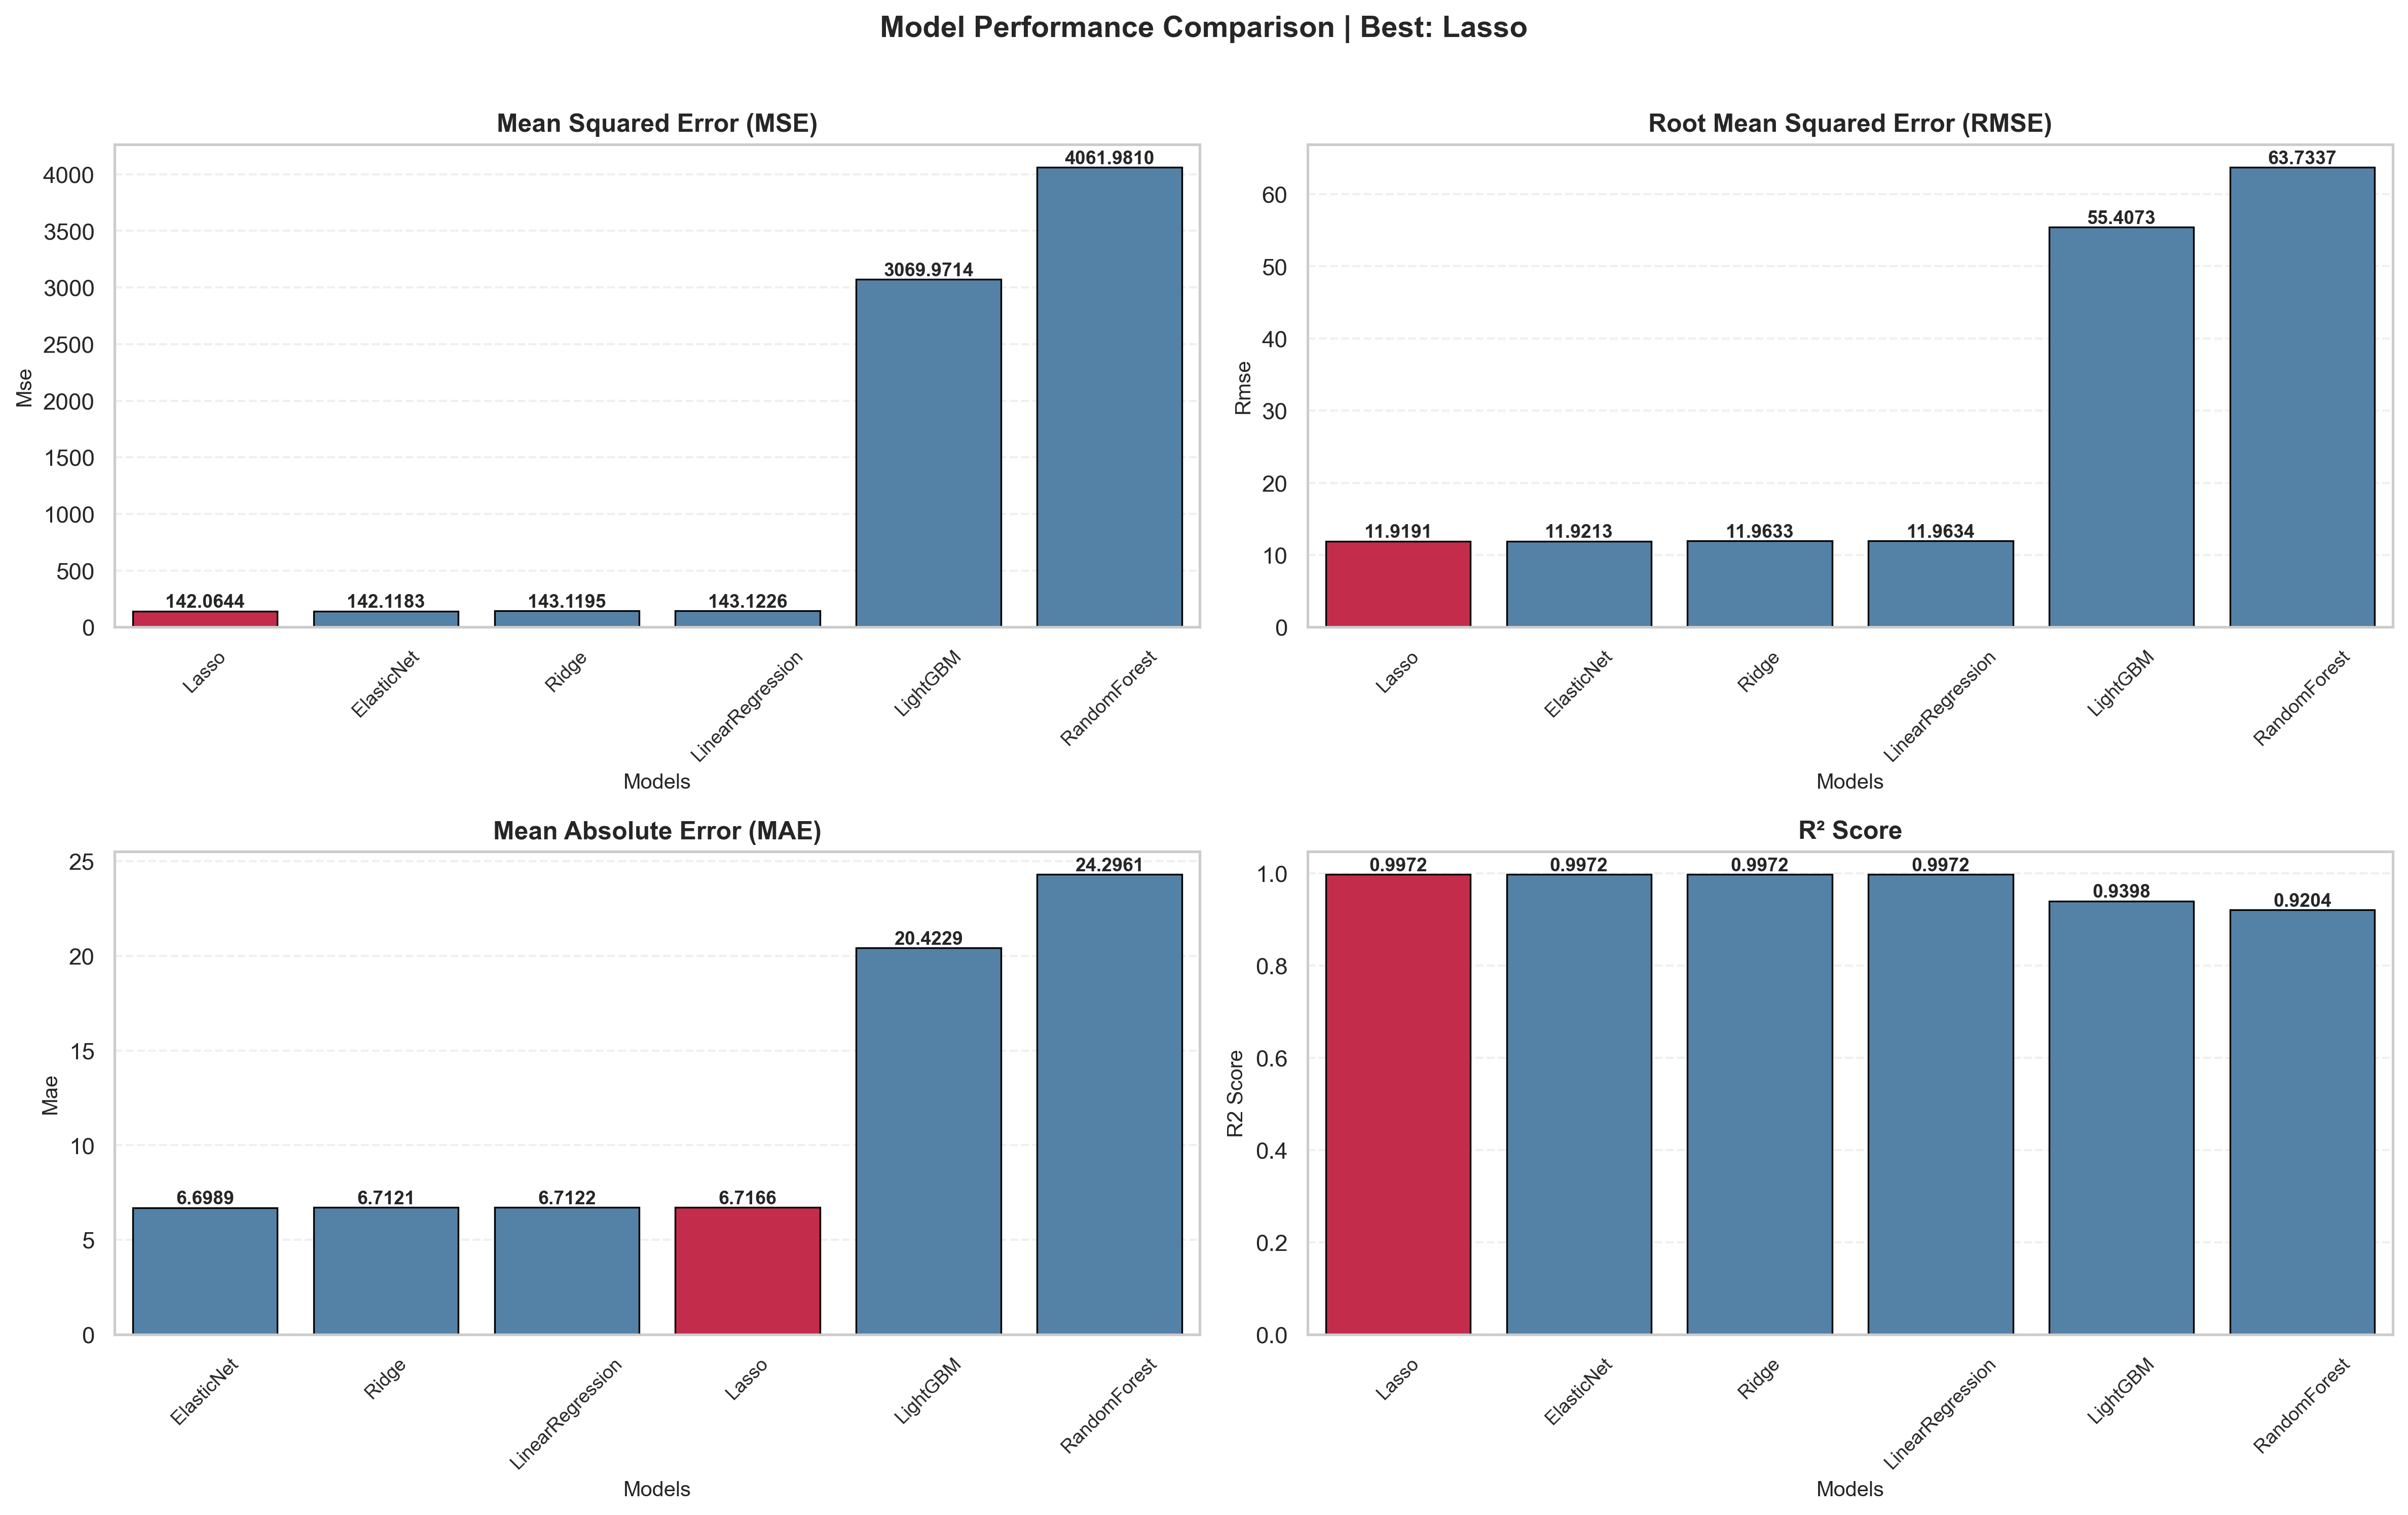
\includegraphics[width=0.75\linewidth]{../../outputs/plots/model_comparison.png}
    \caption{Kết quả so sánh các mô hình học máy trước khi tối ưu siêu tham số}
    \label{fig:compare_models}
\end{figure}

Quan sát Hình~\ref{fig:compare_models}, \textbf{XGBoost Regression} là mô hình có hiệu năng tốt nhất trên cả 4 metrics, với $R^2$ đạt 0.8714 có thể nói rằng mô hình này dự đoán khá tốt với bộ dữ liệu hiện tại.

\begin{figure}[htbp]
    \centering
    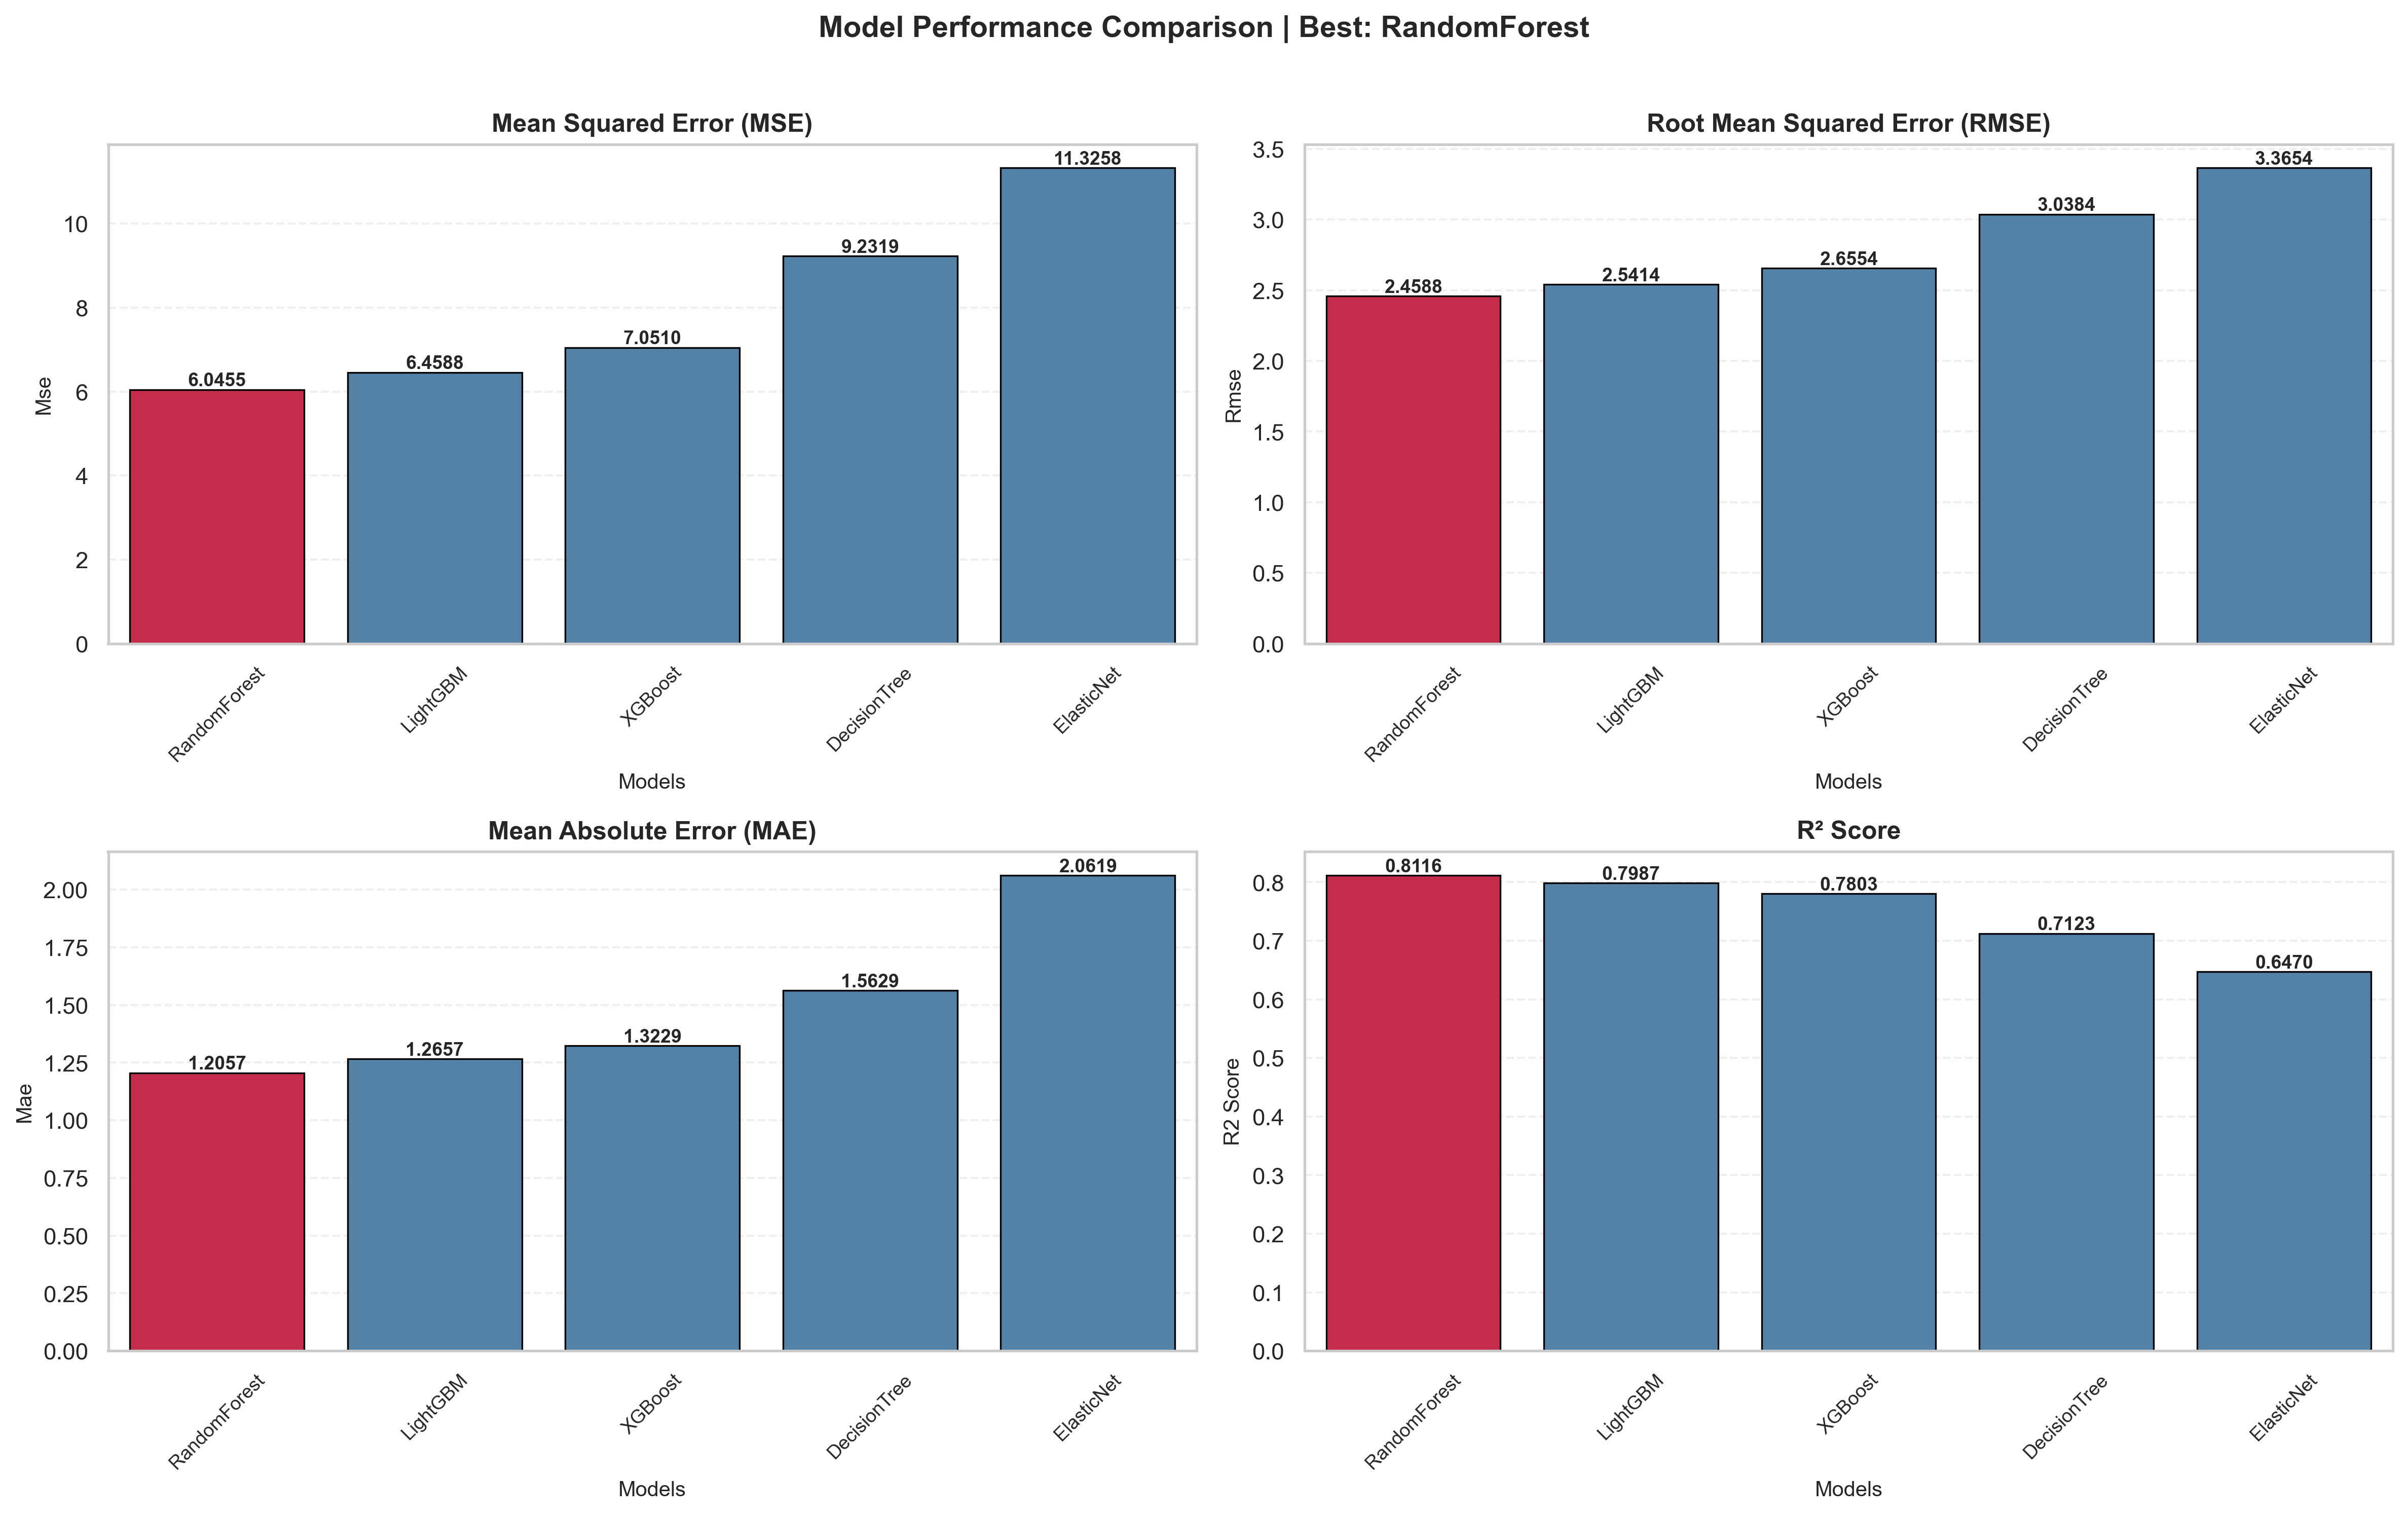
\includegraphics[width=0.75\linewidth]{../../outputs/plots/model_comparison_optimized.png}
    \caption{Kết quả so sánh các mô hình học máy sau khi tối ưu siêu tham số}
    \label{fig:compare_models_optimized}
\end{figure}

Khi thực hiện tối ưu siêu tham số với hàm mục tiêu là tối đa hoá $R^2$, ta thu được kết quả như trong Hình~\ref{fig:compare_models_optimized}. Các mô hình có hiệu suất cao trước khi tối ưu như XGBoost, LightGBM không có sự cải thiện, mô hình Random Forest không hề có sự thay đổi.

\subsection{Phân tích đặc trưng quan trọng của các mô hình}

Kết quả trực quan hoá các đặc trưng quan trọng được thể hiện trong Hình~\ref{fig:all_importance}.

\begin{figure}[H]
    \centering
    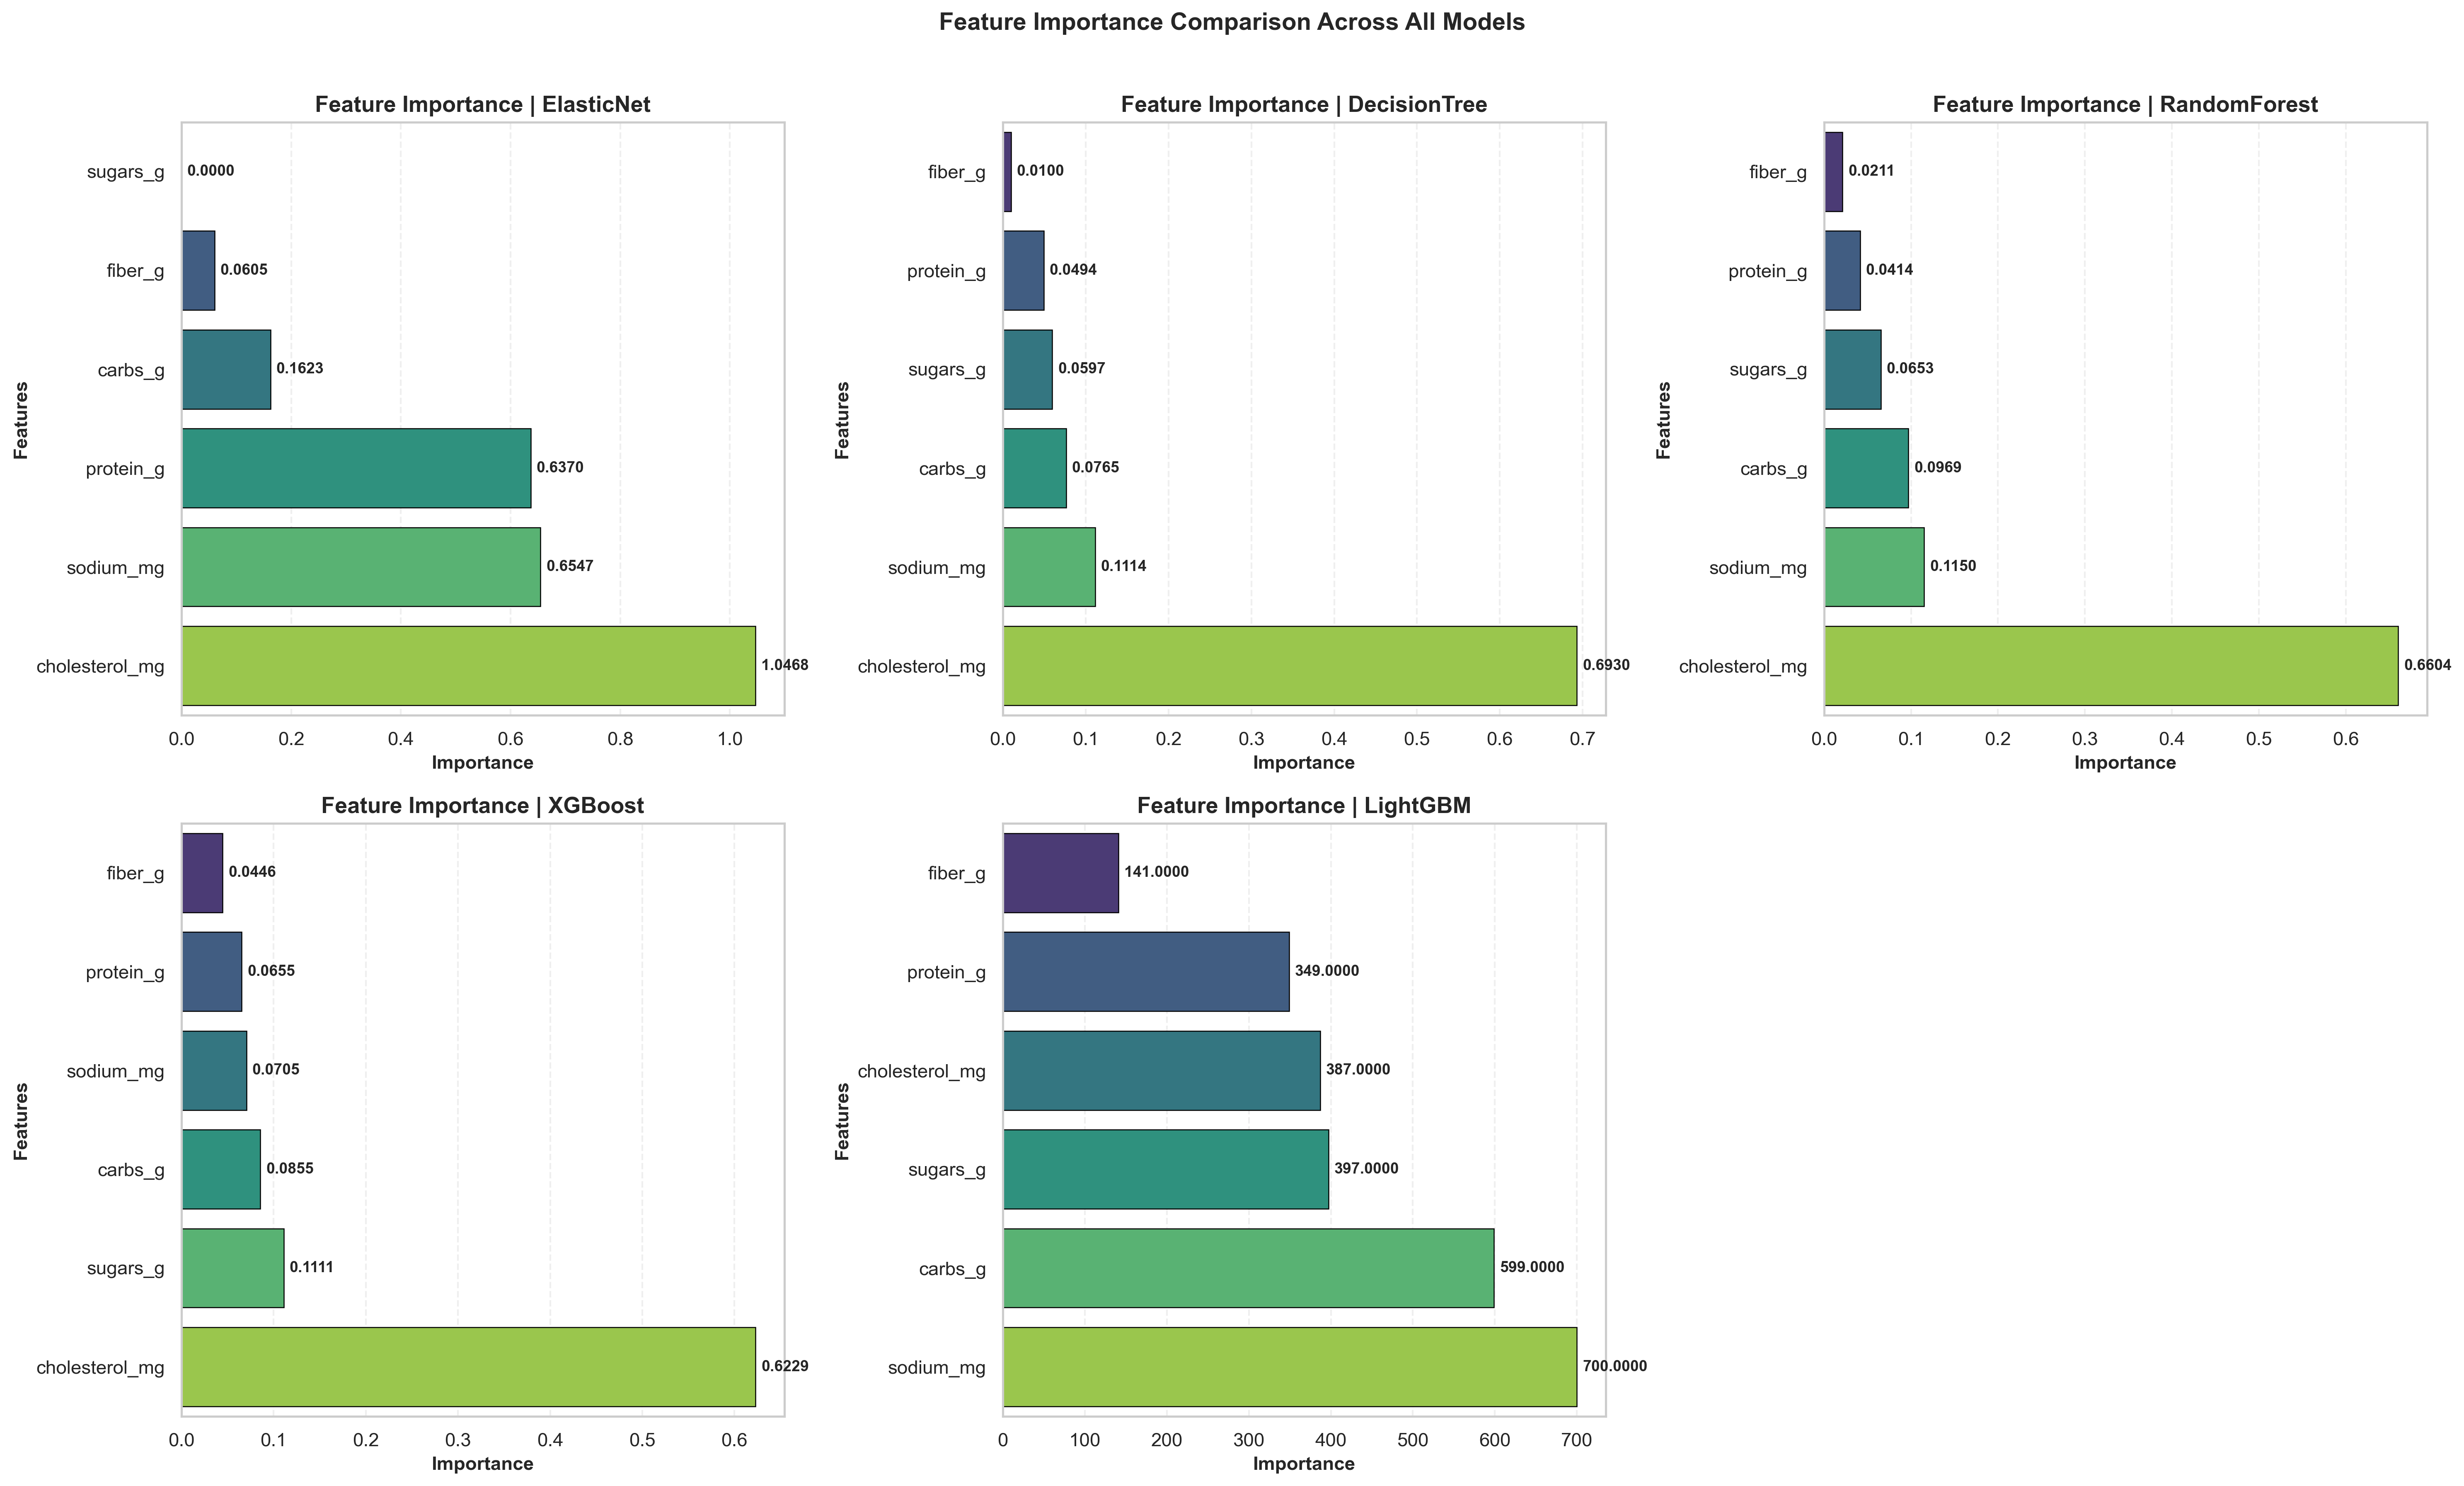
\includegraphics[width=0.9\linewidth]{../../outputs/plots/feature_importance_all_models.png}
    \caption{Các đặc trưng quan trọng theo đề xuất của 5 mô hình trước khi tối ưu}
    \label{fig:all_importance}
\end{figure}

\begin{figure}[H]
    \centering
    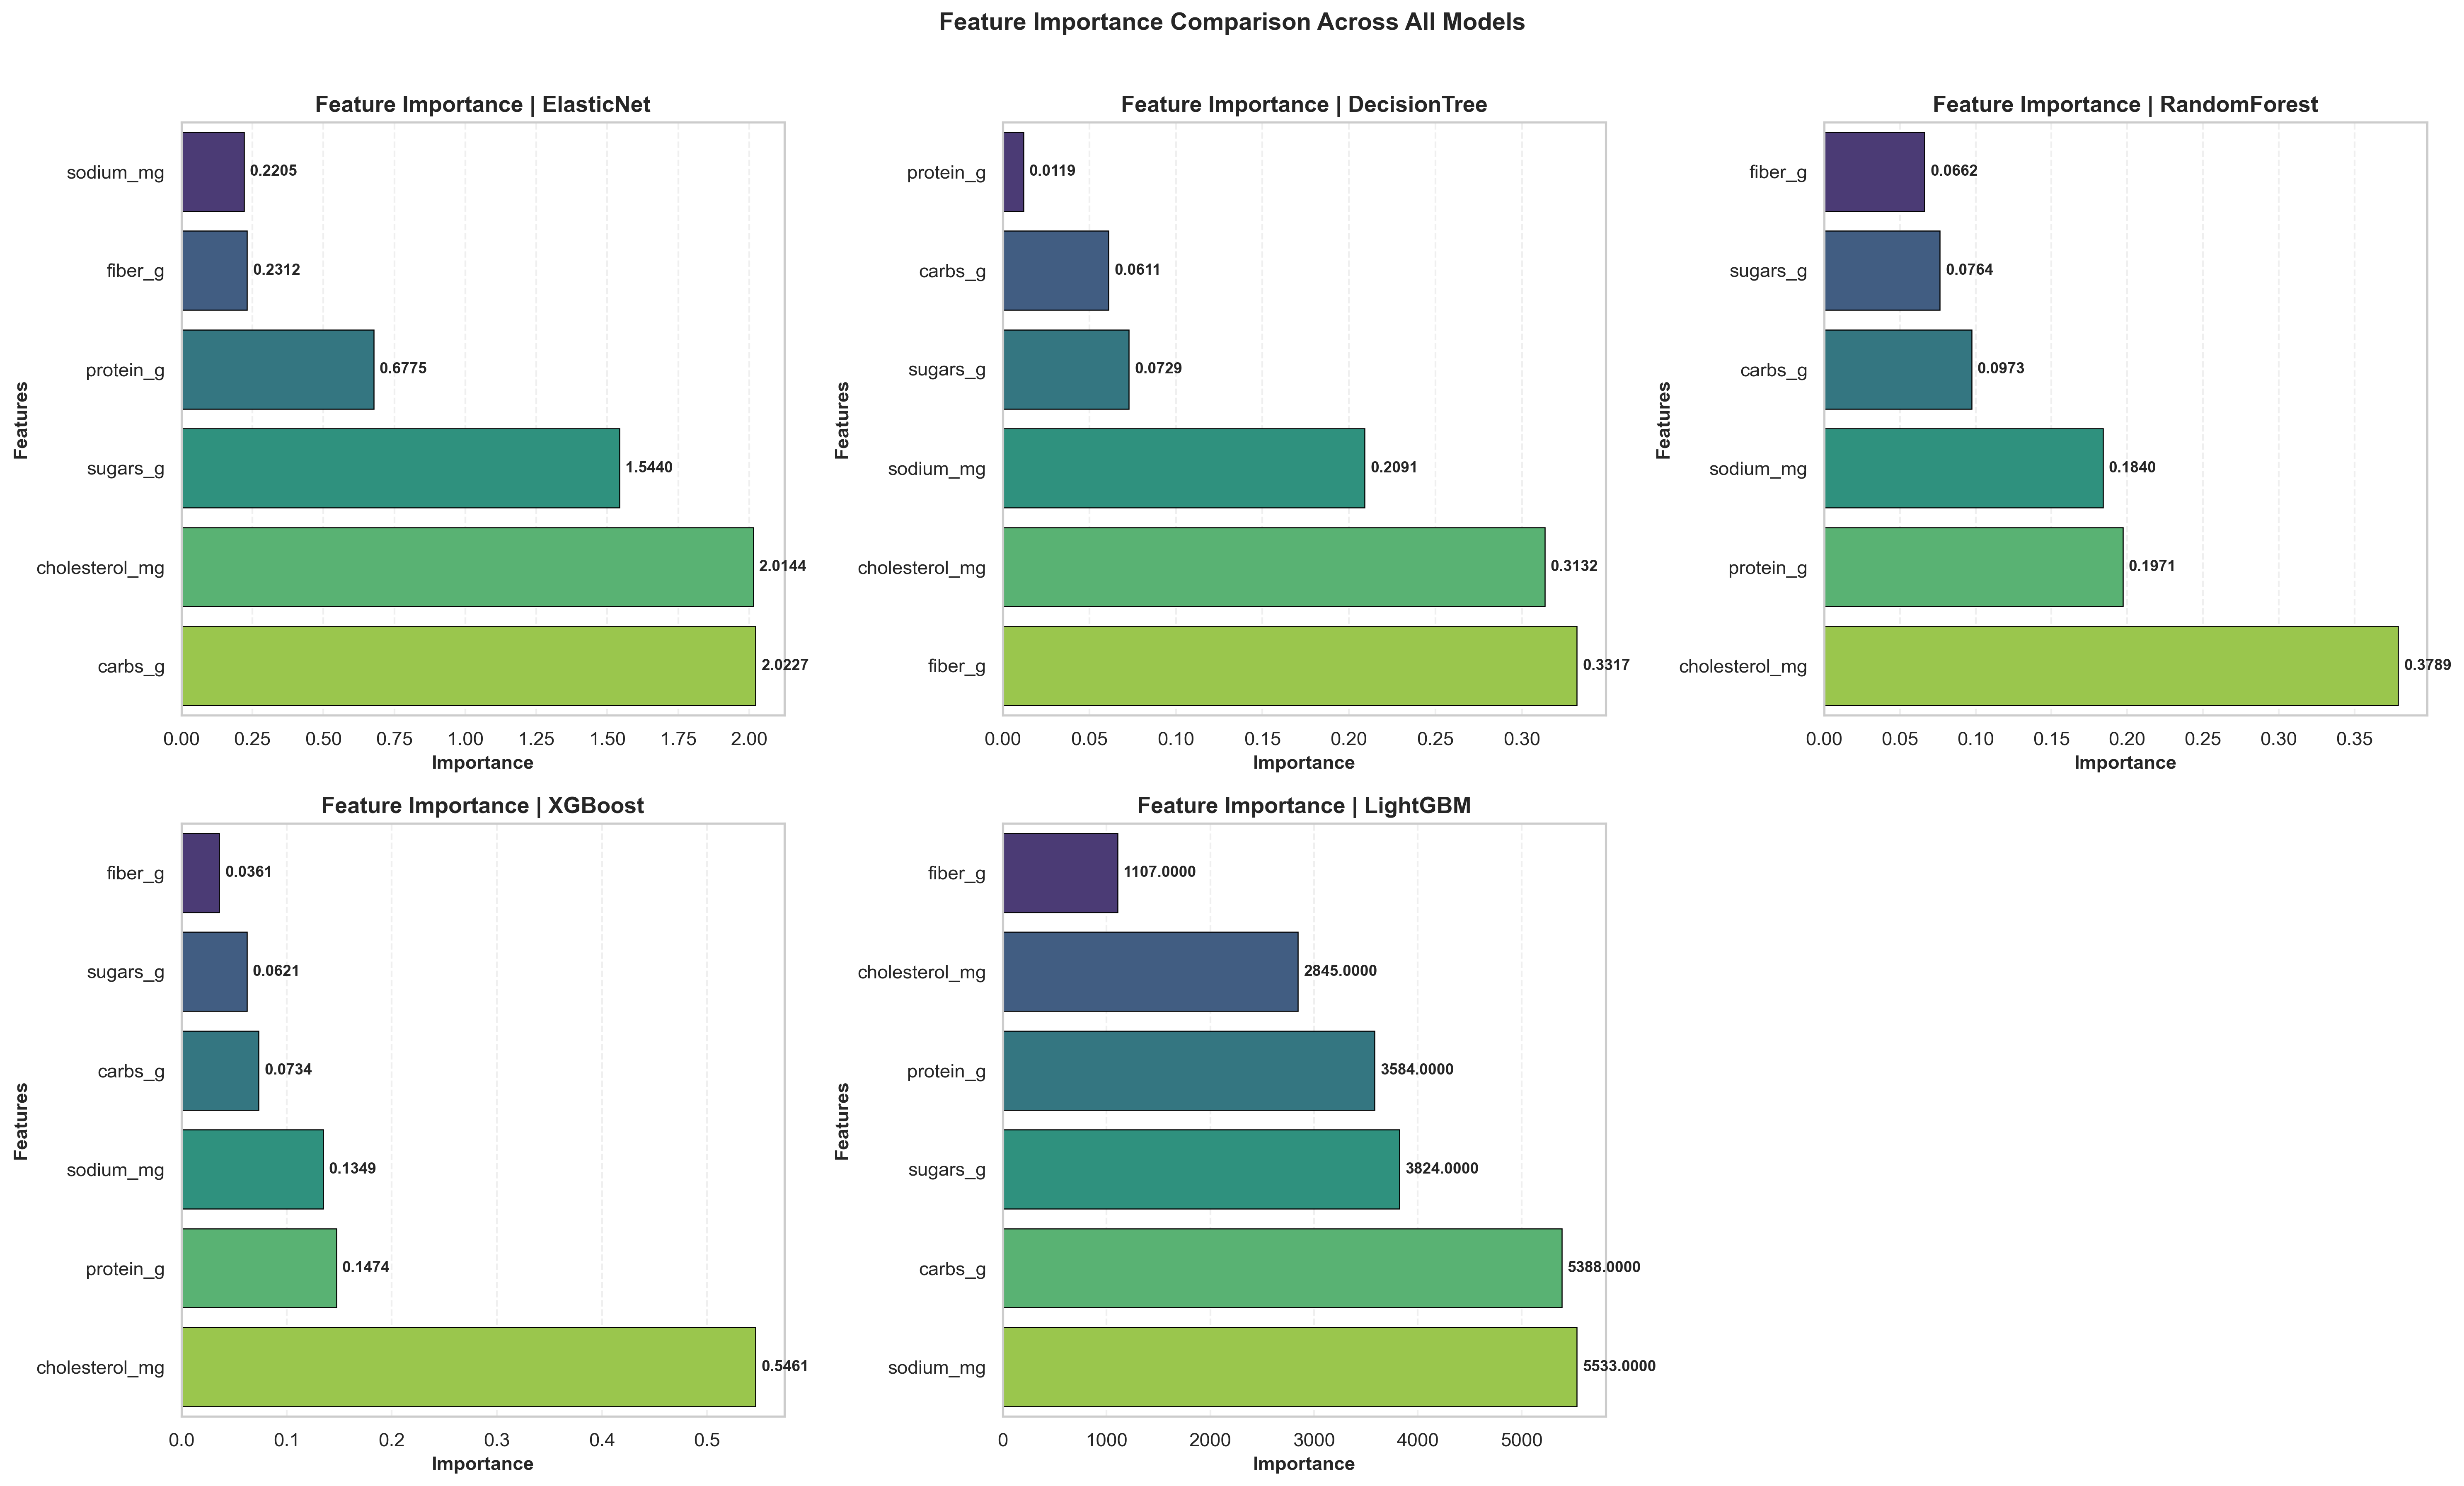
\includegraphics[width=0.9\linewidth]{../../outputs/plots/feature_importance_all_models_optimized.png}
    \caption{Các đặc trưng quan trọng theo đề xuất của 5 mô hình sau khi tối ưu}
    \label{fig:all_importance_optimized}
\end{figure}

Từ Hình~\ref{fig:all_importance}, có tới 4 mô hình đồng thuận rằng các đặc trưng \textbf{cholesterol\_mg} là yếu tố quan trọng nhất ảnh hưởng đến hàm lượng \textbf{saturated\_fat\_g}. 

Mặc dù \textbf{sugars\_g} không có độ tương quan cao với mục tiêu, trái lại được mô hình XGBoost đánh giá là quan trọng gấp 3 lần so với \textbf{fiber\_g} là đặc trưng có tương quan mạnh khi chúng ta phân tích ở Hình~\ref{fig:heatmap_pearson}, Hình~\ref{fig:heatmap_spearman} và Hình~\ref{fig:heatmap_kendall}. Có thể mô hình XGBoost đã phát hiện ra mối quan hệ phi tuyến phức tạp giữa \textbf{sugars\_g} và \textbf{saturated\_fat\_g} mà các mô hình tuyến tính không thể nắm bắt được, do đó nó có kết quả tốt nhất, điều này càng củng cố hơn khi ta phân tích đặc trưng ở Hình~\ref{fig:all_importance_optimized}, \textbf{sugars\_g} được đánh giá khá thấp.

\section{Bảng công việc}

\end{document}
